\chapter{Souborové systémy OS Linux}
%\todo{Srovnani ext3, ext4, udf, fat, ntfs, ... a nastroju pro ně, soustředit se na fsck}
%\todo{Vysvětlit co to je souborový systém?}

\section{Fyzická úložná média}
%\todo{Ozdrojovat...}
Fyzická úložná média představují nejnižší vrstvu  a zároveň základní kámen všech souborových systémů, protože právě na základě jejich vlastností byly vytvářeny.

Z historického hlediska po současnost vývoj přešel přes několik technologií počínaje děrnou páskou a děrnými štítky, přes magnetické ukládání informace do různých nosných médií, optická média po flash paměti. Z hlediska souborových systémů má smysl mluvit až o magnetických médiích, která byla použita pro běžnou práci, protože například lineární pásková úložiště nebyla konstruována pro kompatibilitu s ostatními systémy ale pouze pro vlastní potřeby, tudíž záznam neobsahoval metadata, ale pouze data samotná a jejich struktura byla uložena jinde nebo vůbec. První opravdové použití souborového systému přišlo až s nástupem disket a pevných disků. 

První opravdový souborový systém v Unixu byl \textbf{S5FS} neboli \emph{System V File System} (1974), často ovšem označovaný pouze jako \textbf{FS} (File System) nebo \textbf{UFS} (Unix File System), který byl implementován v \emph{UNIX System V} běžící například na mainframech PDP-11. Tento souborový systém byl velice pomalý a také poměrně jednoduchý, ale právě jeho architektura posloužila jako vzor většiny následujících unixových souborových systémů. Tomu ovšem předcházel souborový systém pro mikropočítače s názvem \textbf{CP/M} (1973) neboli \emph{Control Program/Monitor} a později \emph{Control Program for Microcomputer}. Tento souborový systém byl určen narozdíl od S5FS pro mikropočítače od společnosti Intel. V době vzniku totiž začal Intel vyrábět první osmibitové procesory Intel 8008 a o rok později v roce 1974 vznikl Intel 8080 a právě s ním se rozšířil i CP/M. CP/M byl někde na pomezí mezi souborovým a operačním systémem. Na úložném médiu (v tomto případě disketě) byl BIOS, který poskytoval systémová volání na zápis a čtení, řízení klávesnice a monitoru. Poté bylo CP/M, které využívalo těchto volání a poskytovalo je spolu s dalšími shellu a uživatelskému programu. Systémová volání, která přidalo CP/M se týkaly převážně přístupu k souborům, které CP/M uchovávalo. Dalším významným souborovým systémem, který vznikl pro diskety, byl \textbf{FAT12} (1977). Posléze s rozšířením pevných disků se začaly vyvíjet další nové souborové systémy odpovídající požadavkům.

Z hlediska struktury disku lze mluvit o CHS (\textit{Cylinder-Head-Sector}), které rozdělilo úložné médium ve třech rozměrech podle jednotlivých stop (\textit{Cylinder}), čtecí hlavy (\textit{Head}), kterých může být u pevných disků více, záleží na počtu jednotlivých disků a použitých stran a poslední rozměr je sektor (\textit{Sector}), který určuje, o kterou část stopy jde. Právě sektory dostály ve vývoji největších změn, protože původní dělení po úhlech od středu disku nebylo efektivní se vzrůstající vzdáleností od středu. Proto se později přešlo k dělení na jednotnou velikost sektoru, které se rozložily rovnoměrně po celém disku.

Sektor je nejmenší zápisovou jednotkou na médiu, která je určená výrobcem média. Typicky se jedná o velikosti 512~B u pevných disků, 2048~B u CD-ROM a DVD-ROM. Nové pevné disky používají velikost bloku 4096~B. Důvodem pro členění po sektorech je zjednodušení přístupu k médiu za předpokladu, že uložená data jsou větší než velikost bloku. V opačném případě dochází k plýtvání místem, protože se vždy čte a zapisuje celý blok. Právě proti sektorům se obvykle navrhují bloky souborového systému, které se snaží využít sektory co nejefektivněji jak z hlediska úspory místa, tak z hlediska přístupového a zápisového času.

\section{Diskové oddíly}
Diskové oddíly představují způsob, jak lze fyzické médium abstraktně rozdělit na více částí. Rozdělení na oddíly je uloženo v MBR (Master Boot Record) a jeden disk může obsahovat až 4 hlavní oddíly. V případě potřeby více oddílů lze použít rozšířený oddíl, který zapouzdřuje další dělení na oddíly, ovšem tentokrát již mimo MBR.

Důvodem pro rozdělení na oddíly může být oddělení uživatelských dat od systémových, vyhrazení místa pro odkládací oddíl nebo jiné logické dělení. 

\section{Logical Volume Manager (LVM)}
%\todo{https://wiki.archlinux.org/index.php/LVM}
Logical Volume Manager (LVM) představuje způsob abstrakce nad diskovými oddíly. Ačkoli se může zdát, že se jedná o podobnou technologii jako je RAID, není tomu tak (více v \cite{arch-lvm}).

LVM vzniklo pro zajištění větší flexibility pro organizaci úložiště. Představte si situaci na obrázku \ref{fig:lvm1}. Jedná se o skupinu dvou pevných disků (\texttt{/dev/sda} a \texttt{/dev/sdb}), které jsou z nějakých důvodů, které nejsou podstatné, rozděleny na zobrazené oddíly.

\begin{figure}[] 
    \centering
    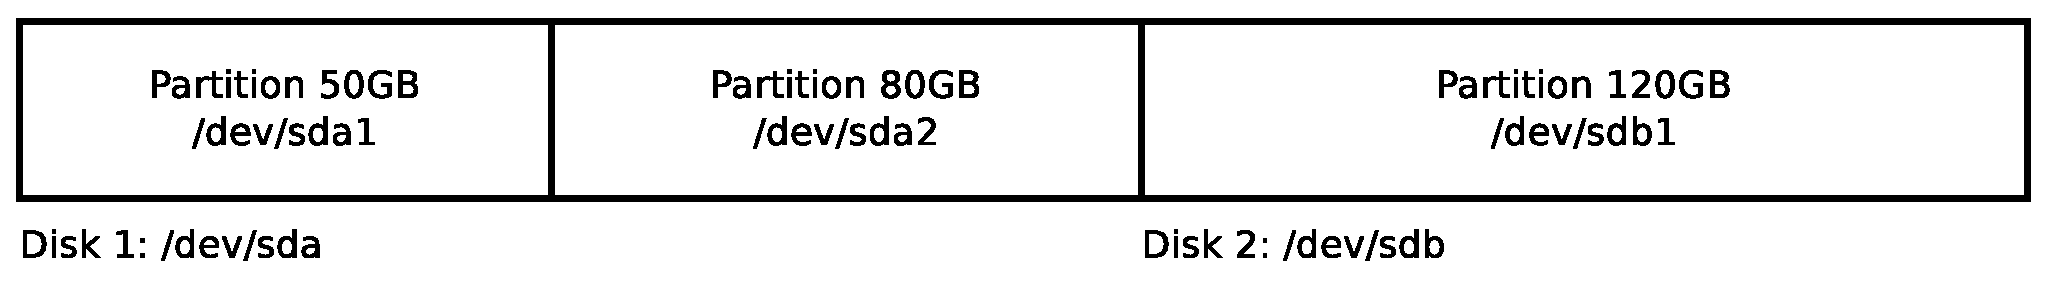
\includegraphics[scale=0.42]{obrazky/lvm1.eps}
    \caption{Výchozí situace z hlediska rozložení diskových oddílů}
    \label{fig:lvm1}
\end{figure}Naším cílem je vytvořit tři diskové oddíly s velikostmi 15~GB, 55~GB a 180~GB. Možnosti jsou dvě. První je RAID~0 a druhou je LVM. Pokud se rozhodneme pro řešení RAID~0, sloučíme disky dohromady do pole a naformátujeme je na požadované oddíly. Totéž můžeme vyrobit i pomocí LVM, jak je naznačeno na obrázku \ref{fig:lvm2}. Řešení pomocí RAID~0 by vypadalo podobně.

\begin{figure}[] 
    \centering
    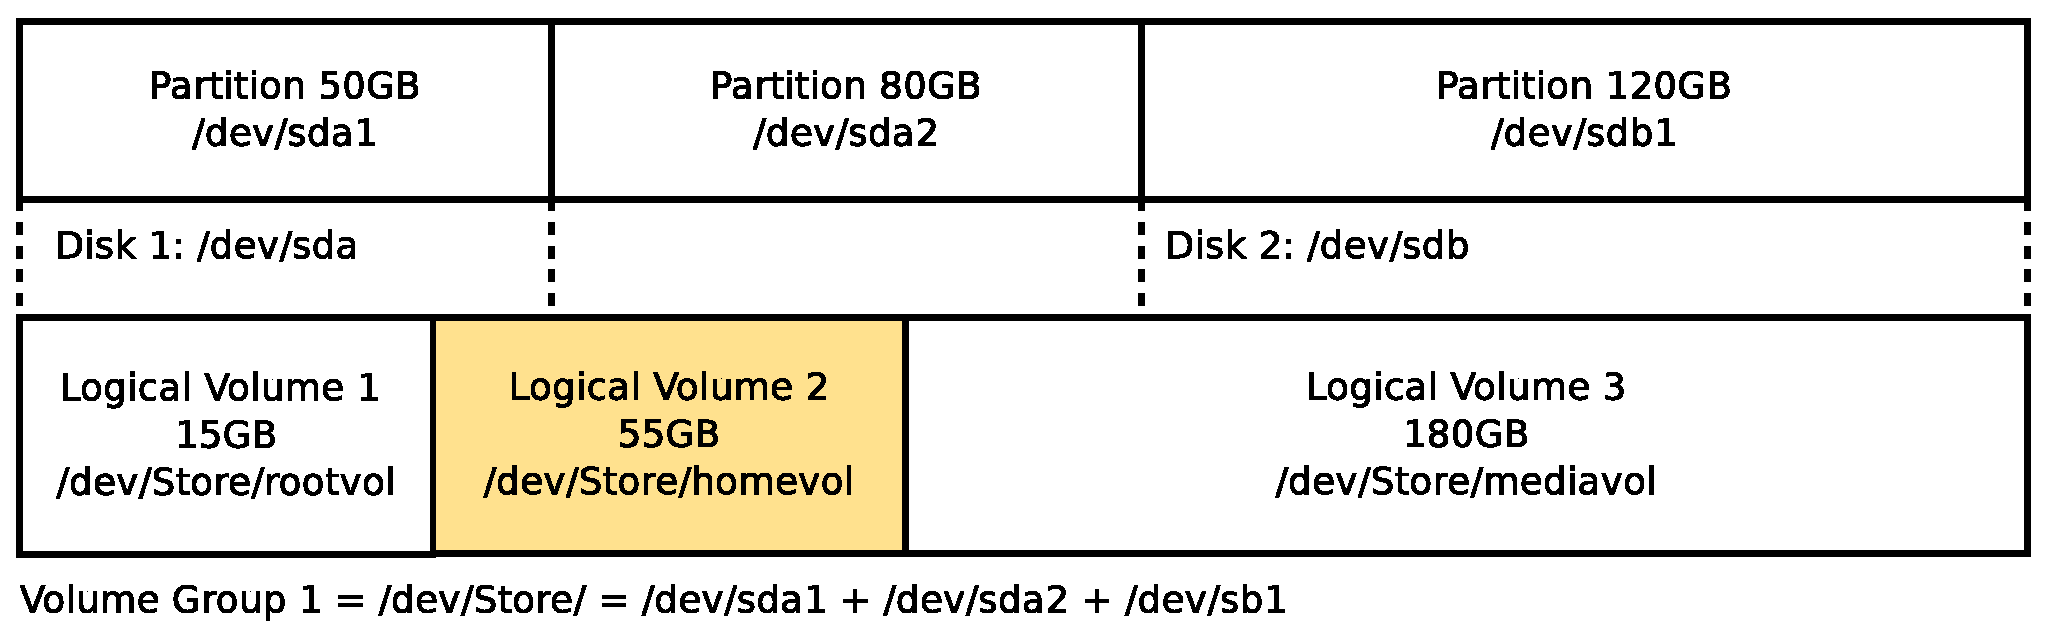
\includegraphics[scale=0.42]{obrazky/lvm2.eps}
    \caption{Namapování diskových oddílů na LVM}
    \label{fig:lvm2}
\end{figure}Pokud se nyní soustředíme trochu více na LVM, můžeme si všimnout, že všechny oddíly byly sloučeny do jednoho logického oddílu \texttt{/dev/Store} s velikostí 250~GB. Tento byl posléze logicky rozdělen na jednotlivé oddíly. Ty mohou poté být naformátovány libovolným souborovým systémem.

Zásadní rozdíl oproti RAID 0 je v možnostech změny struktury úložiště. V případě RAID~0 se změna promítá do formátování RAID úložiště, v případě LVM se jedná o změnu velikosti logické jednotky pouze za předpokladu existence nějakého volného místa, nezávisle na jeho fyzickém umístění na disku. Tudíž není třeba přesouvat oddíly pro potřeby jejich zvětšení. Toto je demonstrováno na obrázku \ref{fig:lvm3}.

\begin{figure}[] 
    \centering
    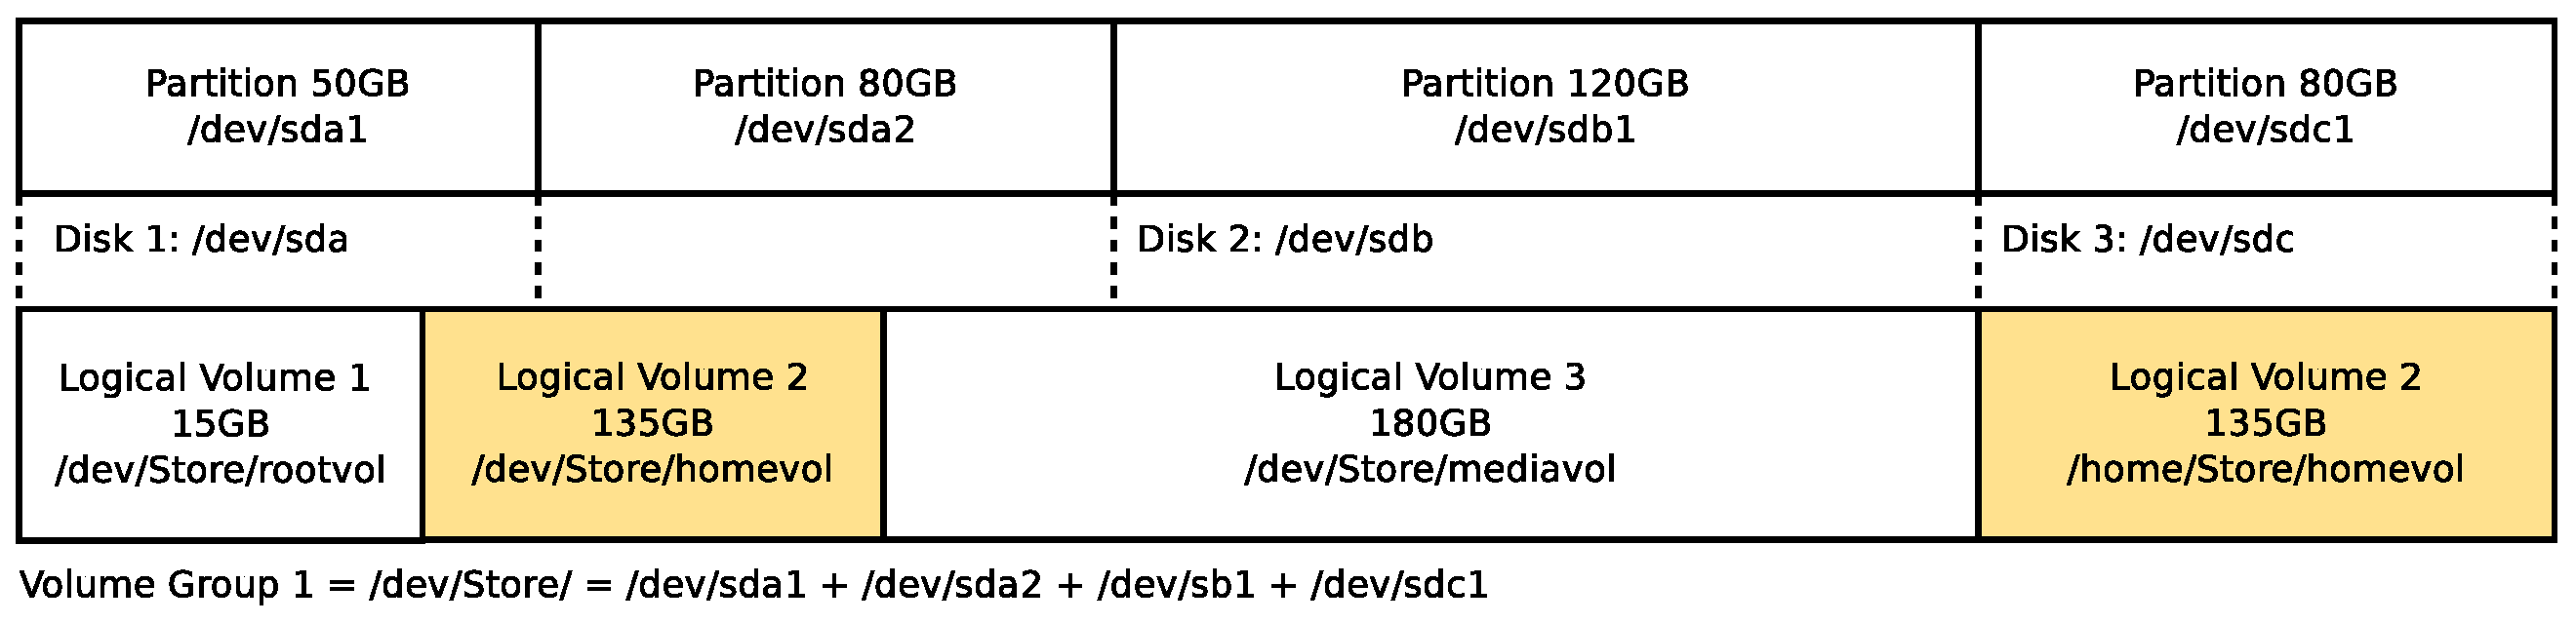
\includegraphics[scale=0.32]{obrazky/lvm3.eps}
    \caption{Ukázka přidání nového disku a zvětšení oddílu na LVM}
    \label{fig:lvm3}
\end{figure}V situaci na obrázku došlo k přidání nového disku \texttt{/dev/sdc} do logického oddílu \texttt{/dev/Store} a přiřazení nově vzniklého místa již existujícímu oddílu. Povšimněte si oranžově zvýrazněného oddílu \texttt{/dev/Store/homevol} na obrázku \ref{fig:lvm2} a nyní na obrázku \ref{fig:lvm3}. Jeho umístění první části zůstalo zachováno a nové místo se pouze připojilo. Stejně tak oddíl \texttt{/dev/Store/mediavol} nebylo třeba přesouvat. Jediný zásah, který je nutný pro používání nového místa, je na straně soubového systému, t.j. jeho zvětšení na celý logický oddíl.

Samozřejmě není nutnost veškeré místo přiřadit pouze jedinému oddílu, místo můžeme dle libosti přiřazovat oddílům, či vytvářet oddíly nové.

Nutno podotknout, že toto řešení nenahrazuje RAID. Ten má stále svou sílu ve svých hardwarových řadičích, tudíž jeho výkonnost je vyšší, ale to je daň za jeho nižší flexibilitu.

\section{Srovnání souborových systémů}
Pro operační systém Linux bylo během jeho existence vyvinuto mnoho různých souborových systémů, stejně tak jako jich bylo mnoho implementováno z ostatních operačních systémů. Některé z nich jsou používány i v současnosti, některé byly opuštěny nebo nahrazeny.

Podle \cite{tldp-filesystem} patří mezi nejvýznamnější nativní souborové systémy tyto:
\begin{itemize}
    \item \textbf{ufs} -- původní souborový systém, který vznikl pro \textit{Unix V}. Posloužil jako vzor pro další vývoj ostatních souborových systémů pro unixové operační systémy. Zavádí pojem \textit{Inode}, který posléze přebírají souborové systémy \textbf{ext}.
    \item \textbf{minix} -- nejstarší souborový systém OS Linux. Vzhledem k jeho stáří se dnes již aktivně nevyvíjí a nepoužívá. Mezi jeho hlavní omezení patří maximální velikost souborového systému, která je až 64~MB. Dalším významným omezením je délka názvů souborů, která je limitována na 30 znaků.
    \item \textbf{ext} -- tento souborový systém, celým jménem Extended Filesystem, vznikl v roce 1992 speciálně pro potřeby kernelu OS Linux \cite{linmag-ext}. Jeho inspirací byl souborový systém UFS (Unix File System), ze kterého převzal strukturu metadat. Jeho limitací byla maximální velikost 2~GB.
    \item \textbf{ext2} -- nástupce souborového systému ext. Byla navýšena maximální velikost na 32~TB a byl navržen podle stejných principů jako Berkeley Fast File System z projektu BSD \cite{nongnu-ext2}. Dlouhou dobu byl tento souborový systém používán ve všech hlavních distribucích OS Linux. ext2 nebyl zpětně kompatibilní s původním ext.
    \item \textbf{ext3} -- již v pořadí třetí verze ext souborového systému. Nyní již byla zachována téměř plná zpětná kompatibilita s ext2. Oproti ext2 ovšem ext3 přineslo žurnálování, které pomohlo v obnově souborového systému při chybě systému \cite{paper-ext3}. Zbytek parametrů zůstal shodný s ext2.
    \item \textbf{ext4} -- současná verze ext souborového systému \cite{paper-ext4}. Opět je zpětně kompatibilní s ext3 a ext2, ale oproti nim byla navýšena maximální velikost na 1~EB, ale doporučené maximum je 16~TB. Původně byl ext4 pouze skupina rozšížení pro ext3, ale později se osamostatnil jako ext4. Dalším rozšířením je nyní již neomezený počet podsložek (ext3 mělo omezení na 32000 podsložek). Také bylo zlepšena odolnost žurnálu přidáním kontrolních součtů a celková výkonnost souborového systému.
    \item \textbf{vfat} -- typický zástupce cizích souborových systémů. V tomto případě se jedná o MS FAT32, který je hojně používaný na USB flash discích.
    \item \textbf{iso9660} -- standardní souborový systém pro CD-ROM. 
    \item \textbf{udf} -- souborový systém původně vyvinutý pro datové rozšíření CD-ROM. Posléze rozšířen pro DVD a BluRay. V současnosti je používán například v šifrovaných flash discích. 
    \item \textbf{smbfs} -- síťový souborový systém Samba File Systém vyvinutý pro sdílení dat mezi počítači s MS Windows. Podporuje Windows Sharing Protocol.
    \item \textbf{ntfs} -- \textit{New Technology File System} je v současnosti nejpoužívanější souborový systém v MS Windows. Jedná se o proprietární souborový systém, který má nativní podporu pouze pro MS Windows. Pro OS Linux vznikla open-source varianta ovladače, která umožňuje jak čtení, tak zápis na \textbf{ntfs}. MacOS má zabudovanou pouze omezenou podporu čtení a zápisu, ale zápis je ve výchozím nastavení zakázán. Zde je možné ovladač dokoupit od třetí strany \cite{paragon-ntfs}.
    \item \textbf{btrfs} -- nový souborový systém založený na principu \textit{copy-on-write} (COW) pro OS Linux. Umonžňuje změnu velikosti souborového systému za jeho běhu, stejně tak přidávání fyzických úložišť. Podporuje kontrolní součty nad daty.
    \item \textbf{hfs} -- proprietární souborový systém vyvinutý společností Apple jako náhrada původního \textit{Macintosh File System}, který vznikl pro diskety a na pevné disky již výkonově nestačil.
    \item \textbf{hfs+} -- náhrada souborového systému \textbf{hfs}, který slouží primárně pro Apple macOS. Opět je proprietární a oproti svému předchůdci podporuje například velké soubory (až 8~EB).
\end{itemize}

\section{Nástroje kontroly integrity}
V prostředí OS Linux je pro kontrolu integrity určen primárně nástroj \texttt{fsck} (Filesystem Consistency Check). V manuálové stránce k \texttt{fsck} \cite{man-fsck} se lze dočíst, že samotný \texttt{fsck} je pouze frontend, který volá specifické nástroje pro daný souborový systém. Skutečné nástroje určené pro kontrolu integrity, které jsou obvykle dodávány spolu s nástroji k vytvoření a práci s daným soborovým systémem, se jmenují \texttt{fsck.fstype}, například \texttt{fsck.ext4}.

Pro masivně používané souborové systémy tyto nástroje existují. Pro \textbf{ext} rodinu se jedná o nástroj \texttt{e2fsck}. Podporovány jsou i převzaté souborové systémy, například \texttt{fsck.fat} pro souborové systémy \textbf{vfat} a \textbf{msdos}. Ovšem například pro \textbf{iso9660} nástroje kontrolující integritu existují pouze jako nástroje vzniklé na základě pokusů při testování vadných disků. Takovým je i \texttt{isovfy} \cite{man-isovfy} ze skupiny nástrojů isoinfo, který ovšem umožňuje pouze kontrolu integrity, nikoli opravu chyb.

Nástrojem, který v tuto chvíli chybí, je podle všeho \texttt{fsck.udf}. Projekt s názvem udftools \cite{udftools-sourceforge}, byl autorem opuštěn v roce 2004 a nástroj pro kontrolu konzistence nebyl nikdy započat a proto se v dalších částech práce soustředím právě na tento souborový systém. 

\chapter{Universal Disk Format}
\label{ch:udf}
\textit{Universal Disk Format} (UDF) je souborový systém navržený pro použití na CD, DVD a Blu-Ray discích, ale díky jeho univerzálnosti je možné jej použít i na jiných médiích. Jeho návrh vyšel ze systému CDFS (ISO~9660). S ním je kompatibilní pouze na úrovni možné koexistence na stejném médiu a ve formátu VRS.

%Jednou z výhod UDF oproti ISO~9660 je například možnost dodatečného zápisu na CD anebo naopak mazání dat z CD a přepisovatelných disků.
Mezi základní vlastnosti UDF patří:
\begin{itemize}
    \item Podpora napříč všemi používanými OS (kompletní výčet je v příloze \ref{ch:podpora}).
    \item Podpora specifických metadat jednotlivých OS na úrovni souborového systému (například \textit{Mac Finder Info}).
    \item Věkem ověřený souborový systém (první verze UDF vznikla v roce 1995, poslední vydaná verze je z roku 2005).
    \item Postavené na mezinárodním standardu ECMA-167/ISO~13346 \cite{ecma-167}. Výsledná specifikace je volně dostupná (specifikace standardu UDF 2.01 \cite{osta-udf-0201}).
    \item Robustní struktura metadat, kritická metadata jsou uložena rednundantně.
    \item Velikost oddílu $2^{32}$ bloků (2~TB pro 512B velikost bloku).
    \item Jména souborů mohou mít délku až 254~B a jsou uložena v Unicode.
    \item Podporuje symbolické odkazy (symlink)
\end{itemize}
Na obrázku \ref{fig:udf-podpora} je zobrazena podpora vybraných souborových systémů ve vybraných operačních systémech. Jak je vidět, pouze UDF a FAT32 jsou jediné, které jsou podporované napříč všemi operačními systémy. Důvodem, proč je UDF nadřazené FAT32, je robustnost celého souborového systému, která je daná návrhem standardu UDF.
\begin{figure}[hb] 
    \centering
    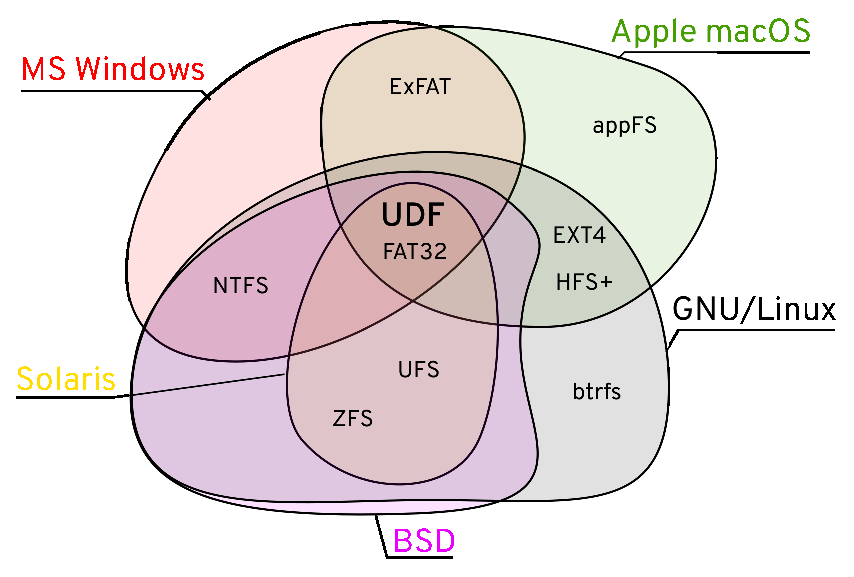
\includegraphics[scale=0.82]{obrazky/udf-podpora.eps}
    \caption{Podpora souborových systémů napříč operačními systémy}
    \label{fig:udf-podpora}
\end{figure}

\section{Historie UDF}
\label{sec:historie-udf}
První verze nového souborového systému \textit{Universal Disk Format} vznikla v roce 1995 ve společenství firem s názvem \textit{Optical Storage Technology Association} (OSTA). Důvody pro vznik nového souborového systému byly hlavně zvyšující se nároky na práci s optickými médii, kde souborový systém ISO~9660 přestával stačit. Jmenovitě se jednalo o blížící se příchod DVD a posléze CD-RW.

Historie verzí UDF v chronologickém pořadí je zachycené v následující seznamu. Jak je vidět, číslování není postupné, toto je kompletní výčet. Mezi jednotlivými verzemi vycházely tzv. DCN dokumenty. Dokumenty s čísly 5100 až po 5122 se týkají UDF standardu a popisují nalezené problémy v jednotlivých verzích UDF a jejich případná řešení. Změny a opravy standardu UDF byly zanášeny na základě těchto dokumentů. Poslední verze je dostupná online \cite{dcn}.
\begin{itemize}
    \item verze 1.00 (24. října 1995) - první vydaná verze
    \item verze 1.01 (3. listopadu 1995) - opravy chyb z verze 1.00, přidán dovětek týkající se použití na DVD-ROM
    \item verze 1.02 (30. srpen 1996) - další opravy verze 1.01, začlěnení DVD-ROM a DVD-Video do specifikace, tato verze byla původně použita pro DVD-Video
    \item verze 1.50 (4. února 1997) - přidána podpora pro CD-R a CD-RW (podpora VAT, správa chyb)
    \item verze 2.00 (3. dubna 1998) - začlenění změn z revize 3 standardu ECMA-167 \cite{ecma-167}, přidání podpory tzv. \textit{Named Streams}, změna fungování VAT
    \item verze 2.01 (15. března 2000) - opravy chyb verze 2.00
    \item verze 2.50 (30. dubna 2003) - přidání \textit{Metadata partition}, navrženo pro HD-DVD a Blu-Ray
    \item verze 2.60 (26. ledna 2005) - přidání pseudo-přepisu pro sekvenční média
    \item verze 2.60 (1. března 2005) - redakční opravy
\end{itemize}
Jak je vidět u verze 2.00, UDF nevzniklo z ničeho, ale bylo vybudováno nad standardem ECMA-167 \cite{ecma-167}, který popisuje jednotlivé deskriptory systému a jejich navrhované použití. UDF přidává svou funkcionalitu do částí popsaných jako \textit{Contents Use}, případně \textit{Application Use}, což jsou části vyhrazené pro konkretizaci použití standardu ECMA-167. V době psaní prvního standardu UDF existovala ECMA-167, revize 2. S revizí 3 vzniklo UDF 2.00 a od té doby nová revize nevyšla. 

\section{Struktura systému}
\label{sec:udf-struktura}
Struktura UDF je naznačena na obrázku \ref{fig:udf-example}. Jak je vidět, obsahuje základní skupiny deskriptorů (jejich popis je v kapitole \ref{sec:deskriptory-udf}) a data. Nutno podotknout, že čísla sektorů jsou pouze ukázková; jediná, která jsou platná jsou sektory 16 (umístění VRS), 256 (umístění AVDP) a poslední sektor (umístění AVDP). Umístění ostatních deskriptorů je závislé na dané implementaci, která vytváří souborový systém.
 
Norma popisující UDF definuje dva druhy číslování. Prvním je \textit{Logical Sector Number} (LSN), které popisuje čísla jednotlivých sektorů. Je číslované od nuly a začíná na prvním fyzickém sektoru média. Jeho velikost odpovídá fyzické velikosti sektoru média. Jeho cílem je fyzická navigace na médiu.

Druhým číslováním je \textit{Logical Block Number} (LBN), které popisuje čísla jednotlivých logických bloků, které jsou mapovány na sektory. Jejich velikost by měla být stejná jako velikost LSN (pokud není, je to v rozporu se standardem UDF). Je číslované od nuly ale začíná až v oblasti dat na začátku logického svazku. Jeho cílem je na rozdíl od LSN navigace pouze v rámci logických svazků.

UDF nese tři příznaky ukazující na jeho stav z hlediska práce s ním. Jedná se o \textit{Access Type}, \textit{Sequentiality} a \textit{Finalization}.

\textbf{\textit{Access Type}} značí možnosti zápisu na médium. Je to údaj uložený v PD (kapitola \ref{subsec:pd-sbd}.) Může být \textit{Read Only} (např. CD-ROM), \textit{Write Once} (např. CR-R, DVD-R), \textit{Rewritable} (např. CR-RW) nebo \textit{Overwritable} (např. DVD-RAM). Tuto informaci musí dodat řadič média. Tento údaj je důležitý pro způsob zápisu na médium. \textit{Read Only} média není třeba řešit, protože zápis nikdy neproběhne. \textit{Write Once} média závisí na stavu \textit{Finalization} - pokud je médium uzavřeno, není možné nic dopsat. Pokud je stále otevřeno, je možné data doplnit, případě mazat (obsazené místo je ale nenávratně obsazené). \textit{Rewritable} média je možné mazat, ale vzhledem k velice omezenému počtu zápisových cyklů není žádoucí zapisovat co není potřeba. Proto se indikuje tento údaj pro omezení zápisů na médium na nutné minimum. To je ostatně také jeden z hlavních důvodů existence \textit{Space Bitmap Descriptor}, aby bylo naznačeno, které bloky je potřeba před dalším zápisem přemazat a které jsou prázdné. Poslední možností je \textit{Overwritable}, tato možnost je určena pro média s ,,neomezeným'' zápisem na médium (neomezeným v porovnáním s CD-RW, například DVD-RAM nebo Flash média.)

\textbf{\textit{Sequentiality}} popisuje, zda je médium sekvenční (například CD-R) nebo nesekvenční (\textit{Random Access}, například Flash disk). Pro sekvenční média totiž UDF poskytuje \textit{Virtal Allocation Table}, která vytváří dojem nesekvenčního (\textit{Random Access}) média.

\textbf{\textit{Finalization}} popisuje, zda bylo vytváření média ukončeno. Jedná se o binární stav, médium je buď ukončeno (\textit{Closed}, případně \textit{Finalized} nebo otevřeno \textit{Open}). Tento stav je odvozen od počtu AVDP uložených na médiu. Pokud je uloženo pouze jediné (na sektoru 256 nebo 512), médium je otevřené (\textit{Open}) a struktura jeho metadat může být ještě měněna v rámci zápisu. Pokud je uloženo AVDP vícekrát (alespoň dvakrát a to na sektorech 256 a buď posledním sektoru ($N$) nebo na sektoru $N-256$), médium je považované za dokončené (\textit{Finalized}).
 
\begin{figure}[] 
    \centering
    %\resizebox{0.5\textwidth}{!}{\input{obrazky/avdp.tex}}}
    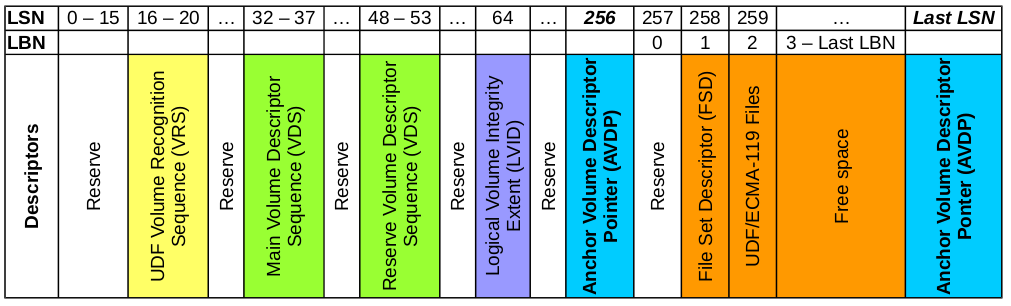
\includegraphics[scale=0.45]{obrazky/UDF-example-schema.png}
    \caption{Příklad struktury UDF}
    \label{fig:udf-example}
\end{figure}

\section{Deskriptory souborového systému UDF}
\label{sec:deskriptory-udf}
Deskriptory souborového systému, neboli metadata souborového systému, jsou klíčovou částí každého FS. UDF používá pět skupin deskriptorů pro svou funkci. Jedná se o tyto:
\begin{itemize}
    \item \textit{Volume Recognition Sequence} (VRS) - oblast definující přítomnost UDF \ref{subsec:vrs}.
    \item \textit{Anchor Volume Descriptor Pointer} (AVDP) - deskriptory ukazující na VDS, vstupní bod do UDF \ref{subsec:avdp}.
    \item \textit{Volume Descriptor Sequence} (VDS) - hlavní skupina deskriptorů popisující UDF. Na souborovém systému je uložena dvakrát \ref{subsec:vds}.
    \item \textit{Logical Volume Integrity Descriptor} (LVID) - deskriptor (případně skupina deskriptorů) popisující integritu souborového systému \ref{subsec:lvid}. 
    \item Deskriptory oblasti dat \ref{sec:file-structure}
\end{itemize}
Vzhledem k velkému překryvu mnou popsaných informací s informacemi, které jsou uvedeny ve standardu UDF~2.01 \cite{osta-udf-0201} a jeho nadřazeném standardu ECMA-167, revize 3 \cite{ecma-167} je tato část pojata pouze jako přehledová a neklade si za cíl absolutně popsat UDF. Cílem je pouze informativně vyzdvihnout důležité deskriptory UDF.

\subsection{Skupina deskriptorů Volume Recognition Sequence}
\label{subsec:vrs}
\textit{Volume Recognition Sequence} (VRS) je sekce určená k rozpoznání obsaženého souborového systému. Může být velká až 6 sektorů a obsahuje deskriptory identifikující souborový systém. Jeho poloha je fixní na sektoru 16.

Důvodem, proč je poloha VRS na sektoru 16, je zpětná kompatibilita a možná koexistence se souborovým systémem ISO~9660. ISO~9660 používá tuto oblast také jako VRS, tudíž je pochopitelné, že ji UDF převzalo. Nese to s sebou i některé výjimky právě kvůli kompatibilitě, například co se týká velikosti sektoru, která je použita v této oblasti. Problematika načítání a zpracování VRS je popsána v kapitole \ref{sec:kontrola-pritomonosti-udf}.

Struktura deskriptorů použitých ve VRS je zachycena v tabulce \ref{tab:vrs}.

\begin{table}
    \centering
    \begin{tabular}{ | l | l | l | l | l | }
        \hline
        Adresa  & Délka [B]   & Jméno položky & Datový typ    & Popis \\ \hline\hline
        0       & 1             & Type           & int8          & Typ deskriptoru \\ \hline
        1       & 5             & Identifier & string        & Identifikátor typu souborového systému \\ \hline
        6       & 1             & Version         & int8          & Verze deskriptoru \\ \hline
        7       & 2041          & ---           & ---           & Volné místo, záleží na typu deskriptoru \\ \hline
    \end{tabular}
    \caption{Struktura VRS deskriptorů\label{tab:vrs}}
\end{table}
Jak je vidět, deskriptor se skládá ze třech částí, pomineme-li poslední rezervovanou část obsahující volné místo. První položka \textit{Type} určuje typ deskriptoru. V tomto případě je jediná povolená hodnota 1. Další položka s názvem \textit{Identifier} obsahuje řetězec o pěti znacích. Tato část určuje typ použitého souborového systému. Možné varianty jsou tyto:
\begin{itemize}
    \item \texttt{BOOT0} - Bootovací záznam
    \item \texttt{CD001} - Souborový systém ISO~9660
    \item \texttt{CDW02} - Souborový systém podle ECMA-168 \cite{ecma-168}
    \item \texttt{BEA01} - \textit{Beginning Extended Area Descriptor}, začátek UDF Bridge sekvence
    \item \texttt{TEA01} - \textit{Terminating Extended Area Descriptor}, konec UDF Bridge sekvence
    \item \texttt{NSR01} - UDF verze 1.00 a vyšší
    \item \texttt{NSR02} - UDF verze 1.50 a vyšší
    \item \texttt{NSR03} - UDF verze 2.01 a vyšší
\end{itemize}
Poslední položkou je \textit{Version} která obsahuje informaci o verzi deskriptoru. Zde by měla být v těchto případech vždy \texttt{0x01}.

Aby mohlo být prohlášeno, že médium obsahuje UDF, musí být nalezen deskriptor obsahující \textit{Identifier} s hodnotou \texttt{NSR01}, \texttt{NSR02} nebo \texttt{NSR03}. V opačném případě se nejedná o UDF.

\subsection{Deskriptor Anchor Volume Descriptor Pointer}
\label{subsec:avdp}
\textit{Anchor Volume Descriptor Pointer} (AVDP) je klíčová část souborového systému. Tato struktura udržuje adresu VDS a jeho délku a to jak pro hlavní, tak pro záložní VDS. Právě AVDP je první deskriptor, který se čte po identifikaci souborového systému, proto je umístěn na předem známém místě. V případě uzavřených souborových systémů (více o \textit{Finalization} v kapiole \ref{sec:udf-struktura}) to je na sektoru 256, posledním sektoru média a nezřídka také na 256. sektoru od konce média. Podmínkou je, že AVDP musí být uloženo alespoň dvakrát. V případě otevřených souborových systémů je zde výjimka, protože AVDP je dočasně umístěno na sektoru 512 nebo 256 až do uzavření média, kdy je dopsáno na svá místa a opět alespoň ve dvou exemplářích, přičemž AVDP na adrese 512 se do tohoto počtu nezapočítává.

Jeho struktura je popsána v tabulce \ref{tab:avdp}. Jak je vidět, obsahuje ukazatele na hlavní a záložní VDS, což zvyšuje robustnost celého souborového systému.
\begin{table}[]
    \centering
    \begin{tabular}{ | l | l | p{4.2cm} | p{1.8cm} | p{5.5cm} | }
        \hline
        Adresa  & Délka [B]   & Jméno položky & Datový typ    & Popis \\ \hline\hline
        0       & 16          & Descriptor Tag & tag        & Popis deskriptoru \\ \hline
        16      & 8           & Main Volume Descriptor Sequence Extent & extent\_ad & Sektor a délka \textit{Main Volume Descriptor Sequence} \\ \hline
        24      & 8           & Reserve Volume Descriptor Sequence Extent & extent\_ad & Sektor a délka \textit{Reserve Volume Descriptor Sequence} \\ \hline
        32      & 480         & Rezerva & & \\ \hline
    \end{tabular}
    \caption{Anchor Volume Descriptor Pointer\label{tab:avdp}}
\end{table}

\subsection{Skupina deskriptorů Volume Descriptor Sequence}
\label{subsec:vds}
\textit{Volume Descriptor Sequence} (VDS) je skupina deskriptorů popisující veškeré vlastnosti souborového systému UDF. Jsou seřazeny postupně na jednotlivých sektorech počínaje adresou udanou z AVDP (viz. kapitola \ref{subsec:avdp}) a končí po počtu logických sektorů uloženém opět v AVDP. Jsou uloženy postupně po sektorech od výchozí adresy a končí \textit{Terminating Descriptor}, což je prázdný deskriptor, který obsahuje pouze \textit{Descriptor Tag}. Samotné pořadí deskriptorů není pevné a samotné deskriptory jsou identifikovány právě pomocí \textit{Descriptor Tag}.

Jak je vidět v AVDP, i tato část je uložena duplicitně pro zvýšení robustnosti. Rezervní VDS je uložena ve stejném tvaru jako primární, tentokrát však od jiné adresy, opět uvedené v AVDP.

Samotné deskriptory jsou popsány ve standardu \cite{osta-udf-0201}, kapitola 2.2. Pro kompletnost zde uvedu jejich výčet ze standardu verze 2.01.
\begin{itemize}
    \item \textit{Primary Volume Descriptor}
    \item \textit{Logical Volume Descriptor}
    \item \textit{Unallocated Space Descriptor}
    \item \textit{Implementation Use Volume Descriptor}
    \item \textit{Partition Descriptor}
    \item \textit{Terminating Descriptor}
\end{itemize}
Z nich je ovšem vhodné některé vyzdvihnout a popsat hlouběji kvůli přímému vlivu na funkci \texttt{fsck}.

\subsubsection{Deskriptor Logical Volume Descriptor}
\label{subsec:lvd}
\textit{Logical Volume Descriptor} (LVD) popisuje logický svazek jako celek. Pro použití ve \texttt{udfffsck} jsou důležité tyto:
\begin{itemize}
    \item \textit{Logical Block Size} - velikost logického bloku svazku. Měla by být shodná s velikostí sektoru. Pokud není, je to v rozporu se specifikací a kontrola není možná.
    \item \textit{Integrity Sequence Extent} - zde je uloženo umístění \textit{Logical Volume Integrity Descriptor} \ref{subsec:lvid}.
    \item \textit{Logical Volume Identifier} - pojmenování logického svazku. Je to řetězec komprimovaného Unicode s maximální možnou délkou 128~B.
    \item \textit{Logical Volume Contents Use} - zde je uloženo umístění \textit{File Set Descriptor} \ref{subsec:fsd}.
\end{itemize}
Struktura deskriptoru je popsána v tabulce \ref{tab:lvd}.
\begin{table}[]
    \centering
    \begin{tabular}{ | l | l | p{4.2cm} | p{1.8cm} | p{5.5cm} | }
        \hline
        Adresa  & Délka [B]   & Jméno položky & Datový typ    & Popis \\ \hline\hline
        0   &16     & Descriptor Tag                    & tag           & Identifikátor deskriptoru \\ \hline
        16  &4      & Volume Descriptor Sequence Number & Uint32        &  \\ \hline
        20  &64     & Descriptor Character Set          & charspec      &  \\ \hline
        84  &128    & \textbf{Logical Volume Identifier}& dstring       & \textbf{Jméno logického svazku} \\ \hline
        212 &4      &\textbf{Logical Block Size}        & Uint32        & \textbf{Velikost logického bloku} \\ \hline
        216 &32     &Domain Identifier                  & regid         &  \\ \hline
        248 &16     &\textbf{Logical Volume Contents Use}& bytes         & \textbf{Umístění \textbf{File Set Descriptor}}\\ \hline
        264 &4      &Map Table Length (=MT\_L)          & Uint32        & \\ \hline
        268 &4      &Number of Partition Maps           & Uint32        & \\ \hline
        272 &32     &Implementation Identifier          & regid         & ID vývojáře a operačního systému, který svazek vytvořil \\ \hline
        304 &128    &Implementation Use                 & bytes         & \\ \hline
        432 &8      &\textbf{Integrity Sequence Extent} & extent\_ad    & \textbf{Umístění LVID} \\ \hline
        440 &MT\_L  &Partition Maps                     & bytes         & \\ \hline
    \end{tabular}
    \caption{Logical Volume Descriptor. Tučně zvýrazněné části jsou kritické pro činnost nástroje pro detekci a korekci chyb.\label{tab:lvd}}
\end{table}

\subsubsection{Deskriptory Partition Descriptor a Space Bitmap Descriptor}
\label{subsec:pd-sbd}
\textit{Partition Descriptor} (PD) popisuje vlastnosti logického svazku. Důležitým údajem je položka \textit{Partition Contents Use}, která popisuje jak se má zacházet s obsahem logického svazku. Obsah logického svazku je definován položkou \textit{Partition Contents}, která může nabývat hodnot uvedených v tabulce \ref{tab:pd-partition-contents}. Další důležitý údaj je v položce \textit{Access Type}, který určuje filozofii přístupu k zápisu na logický svazek (více v kapitole \ref{sec:udf-struktura}.)

Nejdůležitější z vyjmenovaných parametrů je \textit{Partition Contents Use}. Ten v sobě podle \cite{osta-udf-0201}, kapitola 2.3.3 nese \textit{Partition Header Descriptor}, který obsahuje adresu \textit{Unallocated Space Bitmap}, což je \textit{Space Bitmap Descriptor} (SBD).

Ten obsahuje bitový vektor reprezentující logický svazek, kde každý bit odpovídá jednomu logickému bloku. Ten může nabývat dvou hodnot, volný (logická 1) nebo obsazený (logická 0). Spolu s tím je uložen počet bytů a bitů. Tyto dva údaje jsou kritické pro správné fungování bitového vektoru. Důvod je granularita vektoru, která je odvozena od nejmenší možné jednotky a tou je byte, který obsahuje 8 bitů. Tím pádem, pokud oddíl (a potažmo vektor) nemá velikost dělitelnou beze zbytku osmi, zůstanou některé bity v posledním bytu nevyužité. To je nutné indikovat právě počtem bitů. Z tohoto vyplývá, že počet bitů může být buď stejný jako počet bytů nebo nanejvýš o 7 větší.

Důležitost tohoto deskriptoru je při detekci zaalokovaného místa, které není nikde využito, tudíž indikace nedokončeného zápisu.

Struktura PD je zachycena v tabulce \ref{tab:pd}. Struktura SBD je zachycena v tabulce \ref{tab:sbd}. 
\begin{table}[]
    \centering
    \begin{tabular}{ | l | l | p{4.2cm} | p{1.8cm} | p{5.5cm} | }
        \hline
        Adresa  & Délka [B]   & Jméno položky & Datový typ    & Popis \\ \hline\hline
        0   &16     & Descriptor Tag                    & tag           & Identifikátor deskriptoru \\ \hline
        16  &4      &Volume Descriptor Sequence Number  & Uint32        & \\ \hline
        20  &2      &Partition Flags                    & Uint16        & \\ \hline
        22  &2      &Partition Number                   & Uint16        & \\ \hline
        24  &32     &\textbf{Partition Contents}        & regid         & \textbf{Definuje obsah logického svazku} \\ \hline
        56  &128    &\textbf{Partition Contents Use}    & bytes         & \textbf{Obsahuje \textit{Partition Header Descriptor}} \\ \hline
        184 &4      &\textbf{Access Type}               & Uint32        & \textbf{Určuje filozofii zápisu} \\ \hline
        188 &4      &Partition Starting Location        & Uint32        & \\ \hline
        192 &4      &Partition Length                   & Uint32        & \\ \hline
        196 &32     &Implementation Identifier          & regid         & \\ \hline
        228 &128    &Implementation Use                 & bytes         & \\ \hline
        356 &156    &Rezerva                            &               & \\ \hline 
    \end{tabular}
    \caption{Partition Descriptor. Tučně zvýrazněné části jsou kritické pro činnost nástroje pro detekci a korekci chyb.\label{tab:pd}}
\end{table}
\begin{table}
    \centering
    \begin{tabular}{| l | l |}
        \hline
        Obsah & Interpretace \\ \hline\hline
        +FDC01& Médium bylo vytvořeno podle standardu ECMA-107 \\ \hline
        +CD001& Médium bylo vytvořeno podle standardu ECMA-119\\ \hline
        +CDW02& Médium bylo vytvořeno podle standardu ECMA-168\\ \hline
        \textbf{+NSR03}& \textbf{Médium bylo vytvořeno podle standardu ECMA-167/UDF}\\ \hline
    \end{tabular}
    \caption{Partition Contents reprezentace. Zvýrazněný identifikátor je jediný, který nástroj bude podporovat.\label{tab:pd-partition-contents}}
\end{table}
\begin{table}[]
    \centering
    \begin{tabular}{ | l | l | p{4.2cm} | p{1.8cm} | p{5.5cm} | }
        \hline
        Adresa  & Délka [B]   & Jméno položky & Datový typ    & Popis \\ \hline\hline
        0   &16     & Descriptor Tag                    & tag           & Identifikátor deskriptoru \\ \hline
        16  &4      & Number of Bits (=N\_BT)           & Uint32        & Počet použitých bitů \\ \hline
        20  &4      & Number of Bytes (=N\_B)           & Uint32        & Velikost bitmapy \\ \hline
        24  &N\_B   & Bitmap                            & bytes         & Samotná bitmapa \\ \hline
    \end{tabular}
    \caption{Space Bitmap Descriptor\label{tab:sbd}}
\end{table}

\subsection{Skupina deskriptorů Logical Volume Integrity Sequence}
\label{subsec:lvid}
Další důležitou částí je \textit{Logical Volume Integrity Descriptor} (LVID) spolu s \textit{Terminating Descriptor} (TE). Ty dohromady vytváří \textit{Logical Volume Integrity Sequence}. Tato sekvence je uložena pouze jednou a její umístění je udržováno v LVD. Odpovídá na následující otázky:
\begin{itemize}
    \item Je Logický svazek v konzistentním stavu?
    \item Kdy bylo naposledy cokoli na Logickém svazku modifikováno.
    \item Kolik bloků je volných na svazku?
    \item Jaká je celková velikost svazku v blocích?
    \item Byl obsah modifikován nějakou \textit{jinou} implementací od posledního přístupu implementace která svazek vytvořila?
\end{itemize}
Jak je vidět z tohoto výčtu, tato část je důležitá hlavně pro čtení a zápis, ale i pro kontrolu dat má svůj význam, například právě kvůli informaci o konzistenci svazku.
 
Samotný formát struktury LVID je opět v \cite{osta-udf-0201}, kapitola 2.2.6 a v tabulce \ref{tab:lvid}.

Pokud bychom měli zvýraznit některé položky, byly by to tyto:
\begin{itemize}
    \item \textit{Recording date and time} - časová značka posledního záznamu, který byl proveden na médiu.
    \item \textit{Integrity Type} - stav svazku z hlediska probíhajících operací. Může být \textit{Open} (médium je používáno, možný probíhající zápis) nebo \textit{Close} (všechny trasakce byly dokončeny a médium je v konzistentním stavu.)
    \item \textit{Free Space Table} - tabulka popisující volné místo na jednotlivých logických svazcích v logických blocích.
    \item \textit{Size Table} - tabulka popisující velikost jednotlivých logických svazků v logických blocích.
    \item \textit{Implementation Use} - oblast, nepopsaná ve standardu ECMA-167, byla standardem UDF použita k uložení počtu adresářů a souborů uložených na médiu. Dále obsahuje povolené verze UDF pro práci s médiem. 
\end{itemize}
\begin{table}[]
    \centering
    \begin{tabular}{ | l | l | p{3.7cm} | p{1.8cm} | p{4.2cm} | }
        \hline
        Adresa  & Délka [B]   & Jméno položky & Datový typ    & Popis \\ \hline\hline
        0   &16             & Descriptor Tag                    & tag           & Identifikátor deskriptoru \\ \hline
        16  &12             & \textbf{Recording Date and Time}  & timestamp     & \textbf{Časová značka záznamu} \\ \hline
        28  &4              & \textbf{Integrity type}           & Uint32        & \textbf{Otevřené nebo uzavřené médium} \\ \hline
        32  &8              & Next Integrity Extent             & extent\_ad    & Umístění dalšího LVID \\ \hline
        40  &32             & Logical Volume Contents Use       & bytes         &  \\ \hline
        72  &4              & Number of Partitions (=N\_P)      & Uint32        & Počet oddílů \\ \hline
        76  &4              & Length of Implementation Use (=L\_IU)& Unit32     &  \\ \hline
        80  &N\_P$\times4$  & \textbf{Free Space Table}         & Unit32        & \textbf{Tabulka volného místa} \\ \hline
        N\_P$\times4+80$ &N\_P$\times4$& \textbf{Size Table}    & Uint32        & \textbf{Tabulka velikostí} \\ \hline
        N\_P$\times4+80$ &L\_IU& \textbf{Implementation Use}    & bytes         & \textbf{Počet adresářů a souborů a povolených verzí UDF} \\ \hline
    \end{tabular}
    \caption{Logical Volume Integrity Descriptor. Tučně zvýrazněné části jsou kritické pro činnost nástroje pro detekci a korekci chyb.\label{tab:lvid}}
\end{table}

\section{Struktura souborového stromu}
\label{sec:file-structure}
Souborová struktura UDF je postavena na třech deskriptorech, které se podílí na popisu a uložení dat. Jedná se o tyto deskriptory:
\begin{itemize}
    \item \textit{File Set Descriptor} (FSD)
    \item \textit{File Entry} (FE)
    \item \textit{File Identifier Descriptor} (FID)
\end{itemize}
Ty jsou podporovány celou řadou dalších deskriptorů. Z nich je potřeba některé popsat:
\begin{itemize}
    \item \textit{Information Control Block} (ICB) -- deskriptor popisující umístění samotných dat. Jedná se o nadřazené označení pro \textit{File Entry} a \textit{Extended File Entry}. Tuto funkci doplňuje ICB tag, který popisuje metadata ICB.
    \item \textit{Allocation Descriptor} (AD) -- deskriptory popisující umístění v rámci logického svazku. Existují tři varianty: \textit{Short} (ukazauje v rámci logického svazku), \textit{Long} (ukazuje na libovolný logický svazek) a \textit{Extended} (ukazuje na libovolný logický svazek a nese navíc informaci o skutečné délce obsahu, ostatní nesou pouze informaci o počtu použitých bloků.)
\end{itemize}
S touto sadou deskriptorů je již možné popsat strukturu souborového stromu.

\subsection{Deskriptor File Set Descriptor}
\label{subsec:fsd}
\textit{File Set Descriptor} (FSD) je výchozím bodem pro čtení dat. Jeho pozice je opět uložena v LVD (více v kapitole \ref{subsec:lvd}). Jeho struktura je popsána v \cite{osta-udf-0201}, kapitola 2.3.2. Tento deskriptor obsahuje hlavně umístění kořenového adresáře a název svazku, na kterém je uložený. Další údaje uložené v tomto deskriptoru jsou umístění souborů obsahující copyright nebo abstrakt. Ty stojí mimo adresářovou strukturu a jsou využívány například na DVD s filmy.

Kořenový adresář je jediný, který není uveden pomocí \textit{File Identifier Descriptor}, ale přímo pomocí ICB mířícího na \textit{File Entry}. 

\subsection{Deskriptor File Entry}
\label{subsec:fe}
\textit{File Entry} (FE) je deskriptor, který, jak naznačuje název, popisuje jednotlivé záznamy v oblasti dat. Ke každému jednomu souboru nebo adresáři patří jeden FE. Jeho umístění je určeno jeho \textit{rodičovským adresářem}, respektive ji určuje \textit{File Identifier Descriptor}, který je v něm uložen.

Z tohoto pravidla existuje jedna výjimka a to v případě kořenového adresáře. Ten nemá nadřazený adresář (sám je nejvýše umístěný adresář) a jeho pozice je určena přímo pomocí FSD. To s sebou nese druhou výjimku a tou je \textit{Unique ID}. Ta nabývá hodnot 1 až $2^{64}$, přičemž 0 je vyhrazena pro použití před nastavením \textit{Unique ID} a pro kořenový adresář, který jediný musí mít \textit{Unique ID} rovno 0.

Jeho struktura je popsána v \cite{osta-udf-0201}, kapitola 2.3.6, a z ní pouze vyberu některé důležité části.

První důležitou informací je počet zapsaných bloků \textit{Logical Blocks Recorded}. Tento údaj pomáhá vytvořit mapu obsazených sektorů pro srovnání s \textit{bitmap} z SBD \ref{subsec:pd-sbd} a také skutečný počet obsazených sektorů pro srovnání s \textit{Free Space Table} v LVID \ref{subsec:lvid}.

Klíčový údaj pro další práci s FE je rozlišení typu FE. K tomu slouží \textit{ICB tag}, který obsahuje položku \textit{File Type}. Ta může nabývat celé řady hodnot, zajímavé pro nás jsou dvě a to \textit{Directory} a \textit{Regular}. Právě údaj z této části pomáhá rozlišit adresáře od souborů. Další hodnoty jsou speciální druhy záznamů, jako jsou symbolické odkazy, stream adresáře a podobné.
 
Další důležitou částí jsou \textit{Allocation Descriptors}. Velikost této části je určena pomocí \textit{Length of Allocation Descriptors} a obsahuje dva druhy dat, podle toho, jestli se FE popisuje adresář nebo soubor. V případě souboru je v tomto místě uložena pozice dat souboru ve formě \textit{Long Allocation Descriptor} (\texttt{long\_ad}) nebo \textit{Short Allocation Descriptor} (\texttt{short\_ad}). Od adresy uvedené v těchto deskriptorech jsou sekvenčně za sebou ukládána data. V případě adresáře jsou v \textit{Allocation Descriptors} uloženy \textit{File Identifier Descriptor} (kapitola \ref{subsec:fid}), přičemž každý jeden deskriptor nese informaci o jednom \textit{potomkovi} adresáře. Vždy je přítomen nejméně jeden FID a tím je \textit{rodičovský adresář} aktuálního FE.

Zde je opět výjimka týkající se kořenového adresáře. Tou je reference na \textit{rodičovský adresář}, která nemůže vést na FSD, tak je zavedena autoreferenčně na FE kořenového adresáře.

Posledním faktem, který je nutno zdůraznit u deskriptoru FE, je existence novější verze \textit{File Entry} a tou je \textit{Extended File Entry} (EFE). Ta přišla s verzí UDF 2.00 a je doporučené je používat místo FE. Ovšem pro zachování zpětné kompatibility je možné nechat FE na médiu a nadále je používat a nové soubory ukládat pomocí EFE. To s sebou nese nutnost rozlišovat mezi FE a EFE v rámci média, protože EFE pouze nerozšiřuje FE, ale mění i jeho strukturu, takže původní položky jsou sice shodně pojmenované a nesou stejnou informaci, ale mají jiné umístění. 

\subsection{Deskriptor File Identifier Descriptor}
\label{subsec:fid}
\begin{table}[t]
    \centering
    \begin{tabular}{ | l | l | p{3.2cm} | p{1.8cm} | p{4.4cm} | }
        \hline
        Adresa  & Délka [B]   & Jméno položky & Datový typ    & Popis \\ \hline\hline
        0   &16               & Descriptor Tag                    & tag           & Identifikátor deskriptoru \\ \hline
        16  &2                & File Version Number               & Uint16        & Mělo by být nastaven na 1 \\ \hline
        18  &1                & \textbf{File Characteristics}     & Uint8         & \textbf{Charakteristiky souboru (adresář, smazaný atp.)} \\ \hline
        19  &1                & Length of File Identifier (=L\_FI)& Uint8         & Délka jména \\ \hline
        20  &16               & \textbf{ICB}                      & long\_ad      & \textbf{Umístění deskriptoru FE} \\ \hline
        36  &2                & Length of Implementation Use (=L\_IU)& Uint16     &  \\ \hline
        38  &L\_IU            & Implementation Use                & bytes         & Identifikátor poslední implementace, která se souborem pracovala \\ \hline
        L\_IU$+38$&L\_FI      & \textbf{File Identifier}          & d-characters  & \textbf{Jméno v Unicode} \\ \hline
        L\_FI$+$L\_IU$+38$&*  & Padding                           & bytes         & Zarovnání délky na $N \mod 4$ \\ \hline
    \end{tabular}
    \caption{File Identifier Descriptor. Tučně zvýrazněné části jsou kritické pro činnost nástroje pro detekci a korekci chyb.\label{tab:fid}}
\end{table}
\begin{table}
    \centering\label{tab:file-characteristics}
    \begin{tabular}{ | l | l |}
        \hline
        Bit & Význam \\ \hline\hline
        0   & \textbf{Existence} -- Pokud je nastavený, existence souboru by neměla být známá uživateli.\\\hline
        1   & \textbf{Directory} -- Pokud je nastavený, záznam reprezentuje adresář.\\\hline
        2   & \textbf{Deleted} -- Pokud je nastavený, záznam je smazaný.\\\hline
        3   & \textbf{Parent} -- Pokud je nastavený, záznam je rodičovský vůči tomuto.\\\hline
        4   & \textbf{Metadata} -- Pokud je nastavený a je ve \textit{Stream directory}, záznam obsahuje metadata.\\\hline
        5   & Rezervováno, mělo by být rovno 0.\\\hline
    \end{tabular}
    \caption{Význam jednotlivých bitů položky File Characteristics deskriptoru FID \ref{tab:fid}}
\end{table}
\textit{File Identifier Descriptor} (FID) je struktura, která udržuje informace o souboru na úrovni mateřského adresáře. Je popsaný v \cite{osta-udf-0201} v kapitole 2.3.4 a v tabulce \ref{tab:fid}.

Účelem FID je zrychlení přístupu k metadatům souborů na sekvenčních médiích, kde přesun na jiné místo trvá delší dobu než u zařízení s náhodným přístupem (\textit{Random Access}). Takto jsou základní údaje o souboru (adresáři) shluknuty dohromady v rámci rodičovského adresáře a není potřeba je hledat na jiných místech média.

Z deskriptoru FID stojí za zvýraznění \textit{File Identifier}, který udržuje jméno záznamu. Dále se jedná o \textit{File Characteristics}, které popisují vlastnsti záznamu z hlediska práce s ním. Kompletní výčet možností je v tabulce \ref{tab:file-characteristics}. Položka, kterou je také vhodné zmínit, je \textit{Unique ID}. To by mělo být shodné s hodnotou, která je uložená v FE, na které ukazuje. Nejdůležitějším údajem je samozřejmě pozice samotného FE (nebo EFE). Ta je uložena v položce \textit{ICB}. 

\section{Zhodnocení kapitoly}
V této kapitole byly nastíněny základní principy UDF, jeho strukutra a vlastnosti. Protože není cílem popsat existující dokumenty, není výčet kompletní a jedná se pouze o přehledovou část, ve které jsou zvýrazněny části důležité pro kontrolu a opravu konzistence souborového systému.

Výchozímí dokumenty pro tuto kapitolu jsou standardy OSTA UDF do verze 2.01 \cite{osta-udf-0201} a jemu nadřazený standard ECMA-167, revize 3 \cite{ecma-167} z důvodů uvedených v podkapitole \ref{sec:stav-udftools}. Existuje sice novější verze UDF 2.60, ale ta není v práci použita. Veškeré deskriptory byly popsány v duchu těchto dokumentů ve výše zmíněných verzích.


\chapter{Nástroje pro kontrolu konzistence UDF}
\label{sec:nastroje}
Pro OS Linux je znám pouze nástroj \texttt{udfct\_1.5r4}. Tento nástroj byl vyvinut firmou Philips a jedná se o nástroj, který je schopný zkontrolovat integritu souborového systému UDF. Chyby v implementaci UDF a případné chyby v datech vypisuje do terminálu, ale není schopný je opravovat. Zásadním problémem tohoto nástroje je, že existuje pouze pod restriktivní licencí společnosti Philips a není tudíž možné jej využít jako výchozí bod dalšího vývoje i přes dostupnost zdrojových souborů. V současnosti je balíček se zdrojovými kódy dostupný již pouze díky službě Wayback Machine \cite{wayback}, zástupci společnosti Philips jej již nenabízí. Mou žádost o poskytnutí práva na přepoužití jejich kódu ignorovali.

V BSD je \texttt{fsck} v podobném stavu jako v Linuxu ovšem komunita okolo BSD na problému pomalu pracuje. Našel jsem blog \cite{scottuvblog} od Scotta Longa z projektu FreeBSD, kde má shrnutí své práce na UDF včetně jeho patchů do FreeBSD implementace UDF. Mezi jeho body k doplnění je i nástroj \texttt{fsck} a právě proto jsem ho oslovil s prosbou o informace. Právě Scott Long mne odkázal na projekt NetBSD, protože on sám nikdy na \texttt{fsck} nezačal pracovat, ale doslechl se, že v projektu NetBSD něco vzniká. Po hledání jsem nalezl mailing list z roku 2008, kde Reinoud Zandijk popisuje svůj postup práce na UDF implementaci. Na konci jeho zprávy je poznámka o \texttt{fsck} s informací, že bude "brzy". Žádná implementace se ovšem na svět nedostala, takže jsem mu napsal s prosbou o informace o  stavu jeho implementace \texttt{fsck}. Jeho odpověď byla vyčerpávající a potvrzovala mé podezření o stavu open source implementace. On sám má rozpracovanou implementaci \texttt{fsck}, ale zveřejňovat ji zatím nebude, protože není dokončena, jeho slovy: 
\begin{quote} 
    \uv{I've created two UDF implementations: UDFclient \cite{13monkey} and the NetBSD UDF implementation. UDFclient was a kind of study into UDF and far too elaborate to be useful for my FSCK implementation, it'll need to be pruned first.}
\end{quote} 
Nikdo další žádnou jinou open source implementaci nemá vyjma projektu Open Solaris, což bylo panem Reinoudem Zandijkem okomentováno takto:
\begin{quote}
    \uv{As for \texttt{fsck\_udf}, there is only one opensource version and thats the OpenSolaris one. Before you get too excited, its fairly limited and will only check older media and even then only deals with recovering free space and get the directory tree in-order. Important but limited.}
\end{quote}
Implementace v projektu Open Solaris je tedy v současnosti jedinou dostupnou open source implementací \texttt{fsck}. Jejich kód je dostupný na serveru GitHub \cite{solaris-github}. Bohužel ani jejich implementace není kompletní a dokáže obnovit pouze volné místo a strom souborového systému ale bez dat. Dalším omezením je maximální verze UDF, která je omezena na verzi 2.01 ovladačem UDF. Nástroj jako takový exaktní omezení verze nemá. Ovšem i toto je dobrý výchozí bod pro další práci.

Co se týká OSX od společnosti Apple, ti mají nástroje pro kontrolu UDF implementovanou v nástroji \texttt{fsck\_udf} pro všechny existující revize, ovšem zdrojové kódy nejsou veřejně dostupné, takže je možné jejich nástroje použít pouze jako referenční pro srovnání funkčnosti. Druhým nedostatkem je absence jakýchkoli korekcí.

Microsoft Windows má také implementovaný \texttt{CHKDSK} pro UDF, ale jeho zdrojový kód je bohužel uzavřený.


\section{Stav projektu udftools}
\label{sec:stav-udftools}
Projekt udftools byl založen roce 1999 na projektovém serveru SourceForge \cite{udftools-sourceforge} Bennem Fennemou. Byl implementován standard UDF 1.5 a byly vytvořeny nástroje pro paketový zápis na CD, vytvoření souborového systému UDF a pro přístup k němu. Nástroj pro kontrolu konzistence zůstal jako prázdný projekt, byly ovšem vytvořeny nástroje pro vytvoření souborového systému UDF, nástroje pro jeho zápis včetně paketového zápisu (nástroj pro zapisování na CD-R přímo z OS bez nutnosti volat další programy.)

V roce 2007 byly integrovány poslední záplaty a poté projekt zůstal ležet ladem. V roce 2014 byl projekt přemigrován na GitHub \cite{udftools-github} Palim Rohárem a znovu byl započat vývoj, převážně opravy starých chyb. Byla implementována verze UDF 2.01. Nástroj \texttt{fsck.udf} nebyl v tomto projektu nikdy vytvořen a tento stav přetrvává do současnosti.

V tuto chvíli se o projekt udftools stará Pali Rohár, který je správce projektu. Vzhledem k nepříliš vysoké popularitě UDF není projekt udftools aktivní. Sice je stále udržován panem Rohárem, ale aktivní vývoj v tuto chvíli pravděpodobně neprobíhá, nebo alespoň ne veřejně.

Protože bude moje práce navazovat na tento projekt, bude v tuto chvíli maximální možná verze omezena na UDF 2.01, stejně jako zbytek balíčku. Důvodem je sdílená knihovna se zbytkem balíčku obsahující hlavičky deskriptorů, kde by zásah způsobil změny v ostatních nástrojích a také nedostatek testovacích médií ve vyšších verzích.

\chapter{Definice možných chyb souborového systému}
\label{ch:definice-chyb}
%\todo{Jak se to může pokazit? A co se s tím dá dělat?}
Chyby na souborovém systému mohou vzniknout ze třech příčin. 
\begin{enumerate}
    \item Chybou ovladače souborového systému.
    \item Nekorektním odpojením souborového systému (například odpojení flash disku před ukončením všech transakcí).
    \item Fyzickým poškozením média (například stářím poškozené bloky flash paměti nebo poškrábané optické médium).
\end{enumerate}
První druh chyb se děje zřídka. Důvodem je skutečnost, že programy a kernelové moduly starající se o přístup k a práci se souborovými systémy bývají dobře odladěné a otestované. Koneckonců, právě data jsou to, co má v počítačích hodnotu.

Chyby vzniklé nekorektním odpojením souborového systému se vyskytují velice často. Odebrání disku ve spěchu bez korektního odpojení může způsobit poškození souborového systému skrz přerušení probíhající zápisové operace. Systém poté zůstane v nekonzistentním stavu, protože se v něm nachází částečně zapsaný soubor. Případně může dojít k poškození metadat souboru. Do této kateogie spadají i chyby vzniklé havárií operačního systému. Toto riziko se ještě zvýšilo s USB flash disky, kde je velice výrazný vliv vyrovnávacích pamětí jak na straně řadiče, tak na straně disku a i když je disk odebrán ze systému, může ještě probíhat zápis právě z vyrovnávací paměti do flash paměti.

Třetí kategorií chyb jsou veškeré poruchy fyzického média. U optických disků a disket se první vybaví škrábance a rýhy. Tyto chyby poté bývají seskupeny do clusterů poškozených dat. U magnetických disků může dojít k poškození kolizí čtecích hlav s plotnou nebo k poškozením opotřebením.

Existuje určitá prevence některých těchto poruch. Vyšší řady notebooků mají integrovaný akcelerometr a v případě většího zrychlení dojde k nouzovému zaparkování čtecích hlav harddisku. Ovšem ani tato ochrana není absolutní a spíše zabraňuje samotné činnosti disku při pohybu (například při chůzi). Chybám z opotřebení lze předcházet pomocí integrovaného systému S.M.A.R.T., který se stará o sběr telemetrických dat o disku a na jejich základě lze předvídat jeho poruchu (ovšem ani zde není stoprocentní záruka.)

Opravitelnost a analýza chyb je vždy otázkou míry a typu poškození. Od určité míry poškození je oprava buď nemožná, nebo ne úplná. Tuto skutečnost je třeba mít na paměti po celou dobu návrhu opravných algoritmů a je třeba si předem určit, jaký přístup zvolit, zda se spokojíme s částečnou opravou, nebo je oprava vyžadována pouze úplná.

V dále popsané implementaci byl zvolen kompromis, který se spíše přiklání k úplné opravě nebo žádné opravě. Z tohoto jsou vyjmuty pouze deskriptory VDS, které mohou být opraveny jen částečně (t.j. lze pokračovat i s některými deskriptory neopravitelnými.)

\section{Kontrola správnosti dat}
\label{sec:errordetection}
Způsobů, jak detekovat chyby v případě jejich výskytu, je celá řada a liší se požadavky na prostředky a čas. Za naivní přístup lze považovat například detekci porovnáním s referencí. Předpokládejme, že máme stejnou informaci uloženou dvakrát na různých místech (médiích) a v případě poruchy dat je možné data obnovit z referenčního média. Toto řešení je ale evidentně náročné na úložiště kvůli stoprocentní duplicitě dat. Výměnou za to poskytuje informaci nejen o přítomnosti chyby, ale i o její poloze a původních datech. Předpokladem ovšem je znalost, které médium obsahuje data uložená správně.
 
Dalším přístupem je vytváření kontrolních součtů. Tento přístup nám dává oproti předchozímu pouze informaci o přítomnosti chyby bez informace, kde chyba je a jak ji opravit. V extrémním případě se můžou chyby dokonce navzájem vyrušit, takže data nebudou konzistentní, ale kontrolní součet bude stejný. I přes tyto nedostatky je kontrolní součet oblíbená metoda detekce chyb kvůli své jednoduchosti a nenáročnosti na paměť.

Poněkud komplexnější variantou kontrolního součtu je CRC (\textit{Cyclic Redundancy Check}). Tento mechanismus, který původně vznikl pro kabelové přenosy, našel uplatnění všude, kde je potřeba větší šance na detekci chyby než při použití kontrolního součtu. CRC je na výpočet složitější, jeho výstupem je několikabytové číslo a důvodem je větší citlivost na chyby a nižší šance na stejný výsledek při chybě v datech.

Pokud se tyto metody zkonkretizují pro použití na UDF, zjistíme, že jsou použity všechny, ovšem nikoli jednotlivě, ale v kombinaci. To zvyšuje robustnost celého řešení. Tato logika je zachycena na obrázku \ref{fig:detch}. Na obrázku jsou dva deskriptory, hlavní a záložní (případ u VDS). Každý z nich (naznačeno to je pro přehlednost pouze u hlavního) je zabezpečen kombinací CRC a kontrolního součtu následujícím způsobem: Tag, který identifikuje deskriptor, je zabezpečen kontrolním součtem a nese si referenční hodnotu sám v sobě (aby nedošlo k rekurzivní chybě při výpočtu, je místo s referenční hodnotou kontrolního součtu pro jeho výpočet vynecháno). Zároveň zabezpečuje referenční hodnotu CRC pro celé tělo deskriptoru. Pokud je  jak kontrolní součet, tak CRC v pořádku, máme určitou jistotu, že deskriptor není poškozen. Tudíž lze pro obnovu vybrat nepoškozený deskriptor jako vzor, pokud jsou k dispozici dva exempláře.

Nutno podotknout, že toto pouze zajišťuje správnost z hlediska poškození média, nikoli algoritmickou chybu ovladače. Pokud ovladač změní obsah deskriptoru a správně přepočítá CRC a checksum, tento způsob detekce tuto chybu nemůže odhalit.
\begin{figure}[] 
    \centering
    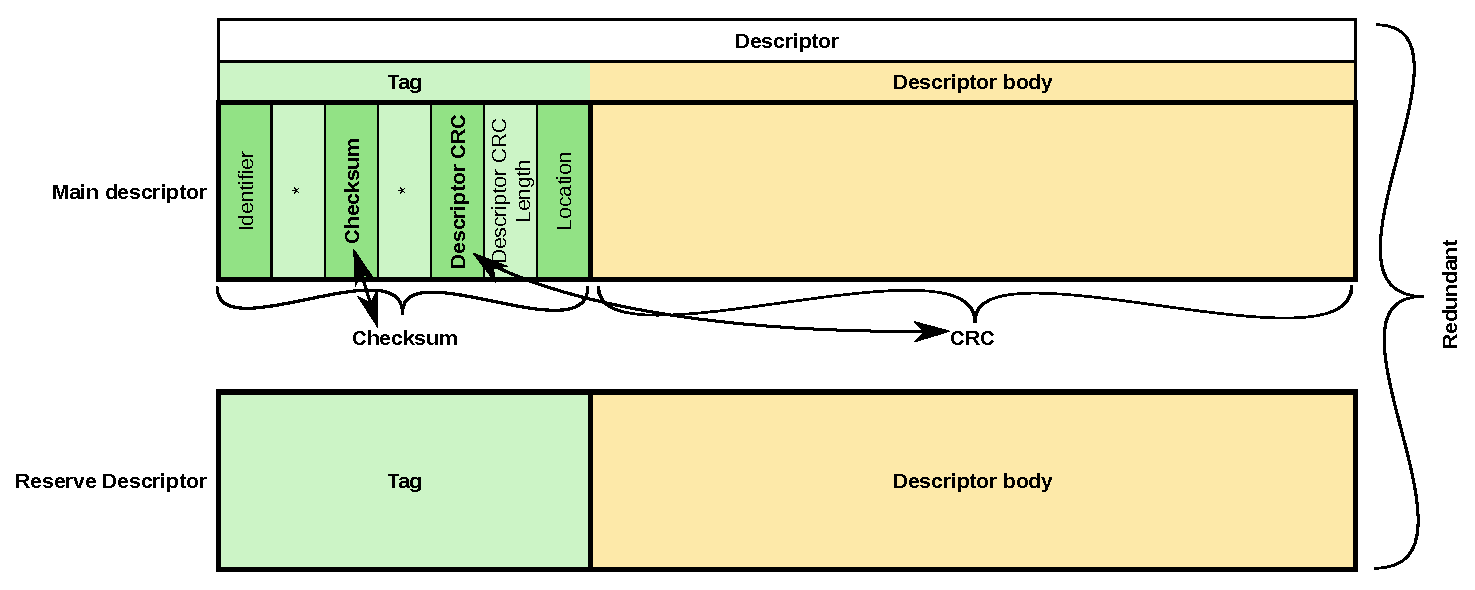
\includegraphics[scale=0.65]{obrazky/det-ch.eps}
    \caption{Schéma kombinace detekčních mechanismů UDF}
    \label{fig:detch}
\end{figure}

\subsection{Zabezpečení pomocí kontrolního součtu}
\label{subsec:checksum}
Zabezpečení pomocí kontrolního součtu (\textit{checksum}) patří k nejzákladnějším kontrolním mechanismům.

Mějme číslenou sekvenci, nad kterou chceme vypočítat kontrolní součet. Postupně přičítejme k výchozí hodnotě (typicky 0) hodnoty z číselné sekvence. Výsledné číslo je kontrolní součet, neboli součet všech hodnot původní sekvence.

V implementaci ve výpočetní technice je toto obvykle realizováno nad sekvencí z nejmenšího datového typu, t.j. nad bytem, který může nabývat hodnot $<0;2^{8}-1>$. Datový typ kontrolního součtu bývá také o velikosti 1~B, ale může být i větší. Pokud hodnota součtu překoná maximální velikost použitého datového typu, výsledek je oříznut na N-bitů a jsou zachovány jeho méně významné bity.

Příklad výpočtu kontrolního součtu pro 5~B dlouhou sekvenci $S=\{10, 25, 130, 221, 85\}$ a 1~B checksum $C$.
V tabulce \ref{tab:checksum-example} je příklad výpočtu nad sekvencí $S$. Kontrolní součet je tedy v tomto případě $C=89$.
\begin{table}[h]
    \centering
    \begin{tabular}{ | l | l | l | l | }
        \hline
        Iterace $i$ & Byte $B$  & \makecell{Kontrolní součet:\\$C_{i}=(C_{i-1}+B) \bmod 256$}  & Popis \\ \hline\hline
        0           & --        & 0                                 & Výchozí stav \\ \hline
        1           & 10        & 10                                & \\\hline
        2           & 25        & 35                                & \\\hline
        3           & 130       & 165                               & \\\hline
        4           & 221       & 4                                 & Zde došlo k přetečení a oříznutí na 8 nižších bitů \\\hline
        5           & 85        & 89                                & Konec výpočtu \\\hline
    \end{tabular}
    \label{tab:checksum-example}
    \caption{Příklad výpočtu kontrolního součtu}
\end{table}

\subsection{Zabezpečení pomocí Cyclic Redundancy Check}
\label{subsec:crc}
\textit{Cyclic Redundancy Check} (CRC) je složitější varianta kontrolního součtu. Matematické odůvodnění jeho funkce je v \cite{crc-prednasky} (přednášky č.6, 7, 8 a 11.)

Důvody pro nasazení CRC oproti kontrolnímu součtu jsou hlavně odolnost vůči chybám vzniklým prohozením bytů, které kontrolní součet z evidentních důvodů nezachytí, zatímco CRC ano. Dalším důvodem je různá výsledná hodnota pro různé délky vstupních dat, přestože jsou všechny vstupní hodnoty nulové.

Ústředním bodem CRC je generační polynom $GP$. Ten určuje, na jaký druh chyb bude CRC citlivé, zdůvodnění opět v \cite{crc-prednasky}. Základní operací, která je při výpočtu CRC použita, je logická operace XOR, která postupně maskuje vstupní sekvenci s cílem ji vynulovat. Z tohoto důvodu je $GP$ vždy zarovnaný nejvíce významným bitem s nejvíce významným bitem dat.

Samotný výpočet je naznačen v tabulce \ref{tab:crc-example}. Je zde aplikován výpočet 4-bitového CRC s generačním polynomem $GP=1 \cdot x^3 + 0 \cdot x^2 + 1 \cdot x^1 + 0 \cdot x^0$, neboli dle koeficientů \textit{GP=1010}. Pro ukázku jsou použita vstupní data \texttt{0100 1011 0001 1111 1100}. Ta jsou rozšířena o délku požadovaného CRC, tedy o čtyři bity s hodnotou 0 (viz. iterace 0 v tabulce.) Podtržená část naznačuje aktuální umístění $GP$, t.j. které bity jsou aktuálně eliminovány.

Na konci výpočtu zbude 4-bitové číslo, které je hledaná hodnota CRC. Detekce, zda došlo k chybě, probíhá stejným způsobem. K datům je připojena část o délce CRC a je vypočítáno znovu. Pokud se výsledky shodují, data jsou v pořádku.

\begin{table}[h]
    \centering
    \begin{tabular}{ | l | l | l | l | }
        \hline
        Iterace $i$ & Vstupní slovo & \makecell{CRC:\\$C_{i}=C_{i-1} \bigoplus GP$(\texttt{1010})}  & Popis \\ \hline\hline
        0           & \texttt{1001} & \texttt{0\underline{100 1}011 0001 1111 1100 0000}         & Výchozí stav \\ \hline
        1           & \texttt{1101} & \texttt{000\underline{1 101}1 0001 1111 1100 0000}         & První XOR s $GP$ \\ \hline
        2           & \texttt{1111} & \texttt{0000 \underline{1111} 0001 1111 1100 0000}         & \\ \hline
        3           & \texttt{1010} & \texttt{0000 0\underline{101 0}001 1111 1100 0000}                & \\ \hline
        4           & \texttt{1111} & \texttt{0000 0000 000\underline{1 111}1 1100 0000}                & \\ \hline
        5           & \texttt{1011} & \texttt{0000 0000 0000 \underline{1011} 1100 0000}                & \\ \hline
        6           & \texttt{1110} & \texttt{0000 0000 0000 000\underline{1 110}0 0000}                & \\ \hline
        7           & \texttt{1000} & \texttt{0000 0000 0000 0000 \underline{1000} 0000}                & \\ \hline
        8           & \texttt{1000} & \texttt{0000 0000 0000 0000 00\underline{10 00}00}                & \\ \hline
        9           & \texttt{1000} & \texttt{0000 0000 0000 0000 0000 \underline{1000}}           & Výsledné CRC\\ \hline
    \end{tabular}
    \label{tab:crc-example}
    \caption{Příklad výpočtu \textit{Cyclic Redundancy Check} s $GP=1 \cdot x^3 + 0 \cdot x^2 + 1 \cdot x^1 + 0 \cdot x^0$}
\end{table}

\section{Použité kontrolní mechanismy v UDF}
\label{sec:kontrolni-mechanismy}
V UDF se využívá několika různých mechanismů, které jsou v případě nutnosti kombinovány pro zvýšení robustnosti. Z obecných mechanismů se jedná o tyto:
\begin{itemize}
    \item redundace dat na médiu,
    \item kontrola deklarované a skutečné polohy deskriptoru,
    \item kontrolní součet (checksum),
    \item robustní kontrolní součet (CRC).
\end{itemize}
V tomto výčtu jsou zachyceny všechny obecné kontrolní mechanismy na úrovni deskriptorů UDF. Kontrolní součty jsou popsány v kapitole \ref{subsec:checksum}, CRC je popsáno v kapitole \ref{subsec:crc}.

Kontrolní součet je použit pro kontrolu \textit{DescriptorTag} a CRC pro kontrolu samotného těla deskriptoru, přičemž jeho referenční výsledek je uložený v již zkotrolovaném tagu. Tento princip je zachycen v kapitole \ref{sec:errordetection}.

Redundance deskriptorů je mechanismus, kterým standard ECMA-167 ošetřil nejdůležitější deskriptory souborového systému a to AVDP (více v kapitole \ref{subsec:avdp}) a skupinu VDS (více v kapitole \ref{subsec:vds}). V případě AVDP byla redundance ještě podtržena fyzickou vzdáleností, kdy je první AVDP uloženo na sektoru 256 a druhý na konci média.

Vedle těchto obecných mechanismů jsou implementovány některé další, konkrétní pro UDF, byť stále vycházející ze standardu ECMA-167.
\begin{itemize}
    \item Použití \textit{Unique ID} pro zabezpečení párovatelnosti metadat souborů k patřičným adresářům. Více v kapitole \ref{sec:filetree}. 
    \item Udržování časových značek indikující poslední práci se souborovým systémem. Více v kapitole \ref{sec:nacteni-a-oprava-lvid}.
    \item Značka v položce \textit{Integrity Type} indikující probíhající zápisovou operaci na médium. Více v kapitole \ref{sec:nacteni-a-oprava-lvid}.
    \item Pořadí operací pří zápisu na médium.
\end{itemize}
Pořadí úkonů zápisové operce na médium je toto:
\begin{enumerate}
    \item Nastavení probíhající zápisové operace v LVID \textit{Integrity Type} na \textit{Open}.
    \item Kontrola a změna objemu volného místa v \textit{Free Space Table} a v SBD.
    \item Zvýšení počtu souborů / adresářů v LVID.
    \item Spuštění zápisu dat na médium.
    \item Po dokončení zápisu se vytvoří \textit{File Entry} s patřičným \textit{Unique ID} a časovou značkou. 
    \item Vytvoření nového \textit{File Identifier Descriptor} v rodičovském adresáři a svázání s FE.
    \item Ukončení zápisové operace nastavením \textit{Integrity Type} na \textit{Close}.
\end{enumerate}
Toto pořadí úkonů zajišťuje, že při přerušení zápisu dat zůstane systém v nekonzistentním stavu a bude možné detekovat, že zápis byl nekorektně přerušen.

\chapter{Realizace nástroje pro detekci chyb}
\label{ch:realizace}
Nástroj \texttt{udffsck} vznikal ve dvou fázích. V první fázi byl navržen a implementován nástroj určený pouze k detekci chyb na UDF. Ten byl ve druhé fázi rozšířen o opravy nalezených chyb. Postup návrhu a následné implementace je popsán v následujcích podkapitolách.

\section{Návrh nástroje pro detekci a korekci chyb}
\label{sec:navrh}
Návrh nástroje byl rozdělen do dvou částí a to na návrh detekce chyb a návrh jejich korekce.

Vzhledem k faktu, že UDF existuje již řadu let a během té doby se postupně vyvíjelo, existuje celá řada potíží, které sebou UDF nese ve svých implementacích na různých platformách. Obvyklou příčinou je nedoimplementovaná nějaká oprava specifikace, která vyšla až po vydání daného nástroje. Otázkou je, jak nakládat s médiem, které trpí těmito problémy. Varianty jsou dvě: opravit podle poslední platné verze nebo nechat tyto problémy být, vzhledem k faktu, že se nejedná o provozní chyby, ale o chyby vůči specifikaci.

Byl zvolen benevolentnější přístup a to chyby vůči specifikaci, které vznikly až na základě oprav specifikace, neopravovat. Důvodem je častá nemožnost je opravit úplně. Typickým příkladem takovéto chyby je vyhrazená velikost deskriptoru LVID, který podle specifikace 2.01 má mít velikost 2048~B ale podle pozdějších dokumentů je doporučená velikost 8192~B. Problém je, že ne každé médium má místo pro umístění většího deskriptoru a poté není oprava možná. Proto byl tento druh chyb prozatím vynechán.

Chyby, které jsou detekovány vždy, jsou chyby v kontrolních mechanismech deskriptorů (jmenovitě kontrolní součet, CRC a umístění deskriptoru). Další druh chyb vzniká během nesprávného odebrání média. Těmi jsou chyby založené na mechanismech v kapitole \ref{sec:kontrolni-mechanismy}, což jsou jmenovitě chyby typu neuzavřené médium, nenastavené nebo neshodující se \textit{Unique ID}, špatná časová značka v deskriptoru souboru nebo v LVID. Tyto chyby jsou taktéž detekovány a považovány za chyby. Poslední druh chyb, které jsou detekovány, jsou neshodující se údaje o obsazeném a volném místě na médiu jednak z hlediska jeho velikosti a jednak z hlediska jeho umístění.

Na základě těchto požadavků vznikla struktura programu pro detekci těchto chyb. Její zjednodušená strukutura je zachycena na obrázku \ref{fig:steps-detekce}.
 
\begin{figure}[h] 
    \centering
    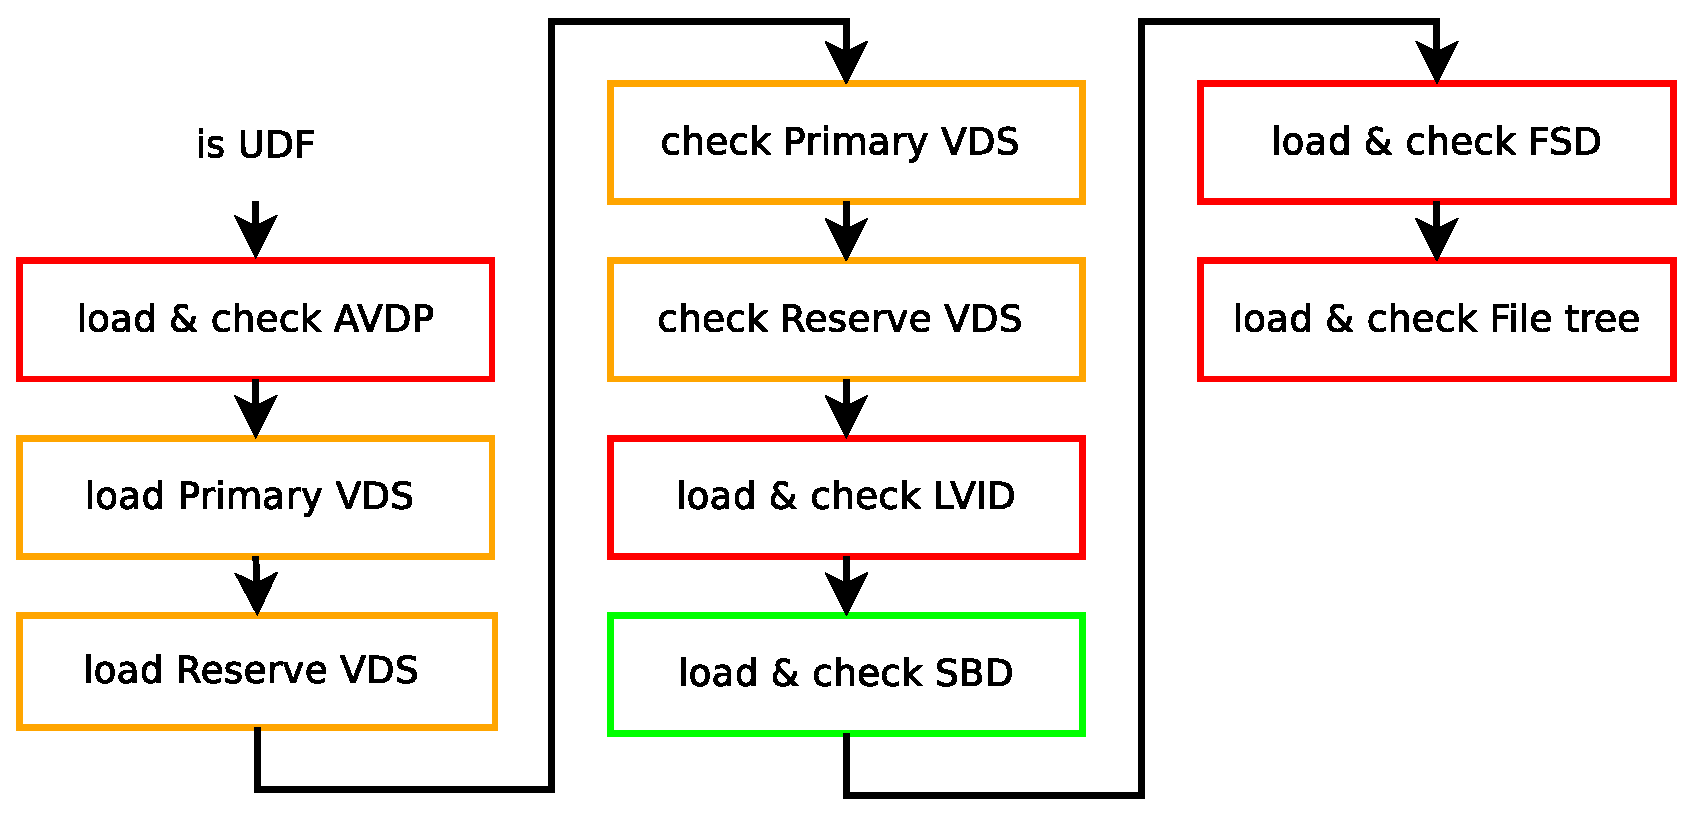
\includegraphics[scale=0.4]{obrazky/steps1b.eps}
    \caption{Zjednodušený algoritmus detekce}
    \label{fig:steps-detekce}
\end{figure}
Zjednodušená z toho důvodu, že v ní není zachycena počáteční detekce velikosti sektoru a průchod stromem souborů je zjednodušen na jedinou operaci. Obecně se pod \textit{Load} rozumí načtení deskriptoru z média do operační paměti a pod \textit{Check} kontrola všech výše zmíněných chyb, pokud jsou v daném kroku aplikovatelné.

V algoritmu jsou kroky barevně rozlišeny do třech kategorií podle důležitosti, respektive podle jejich vlivu na další činnost pokud jejich načtení nebo kontrola selže. Červené kroky jsou kritické pro činnost a jejich selhání znamená selhání programu. Oranžové kroky jsou závislé na míře poškození. Pokud v PVD bude alespoň od každého druhu jeden deskriptor v pořádku, je možné pokračovat. Zelené kroky je možné vynechat, ale může to být na úkor některých detekcí (v případě SBD by byla vynechána kontrola rozložení obsazeného místa).

Návrh algoritmu pro korekci spočíval v navázání na existující detekční algoritmus. To spočívalo ve vytvoření mechanismu pro předání nalezených chyb druhé části algoritmu a způsobu jejich opravy. Tato část byla myšlenkově rozdělena opět na tři části a to na opravu deskriptorů jako takových, opravu volného místa a opravu stromu souborů. Struktura algoritmu korekce je zachycena na obrázku \ref{fig:steps-korekce}
\begin{figure}[h] 
    \centering
    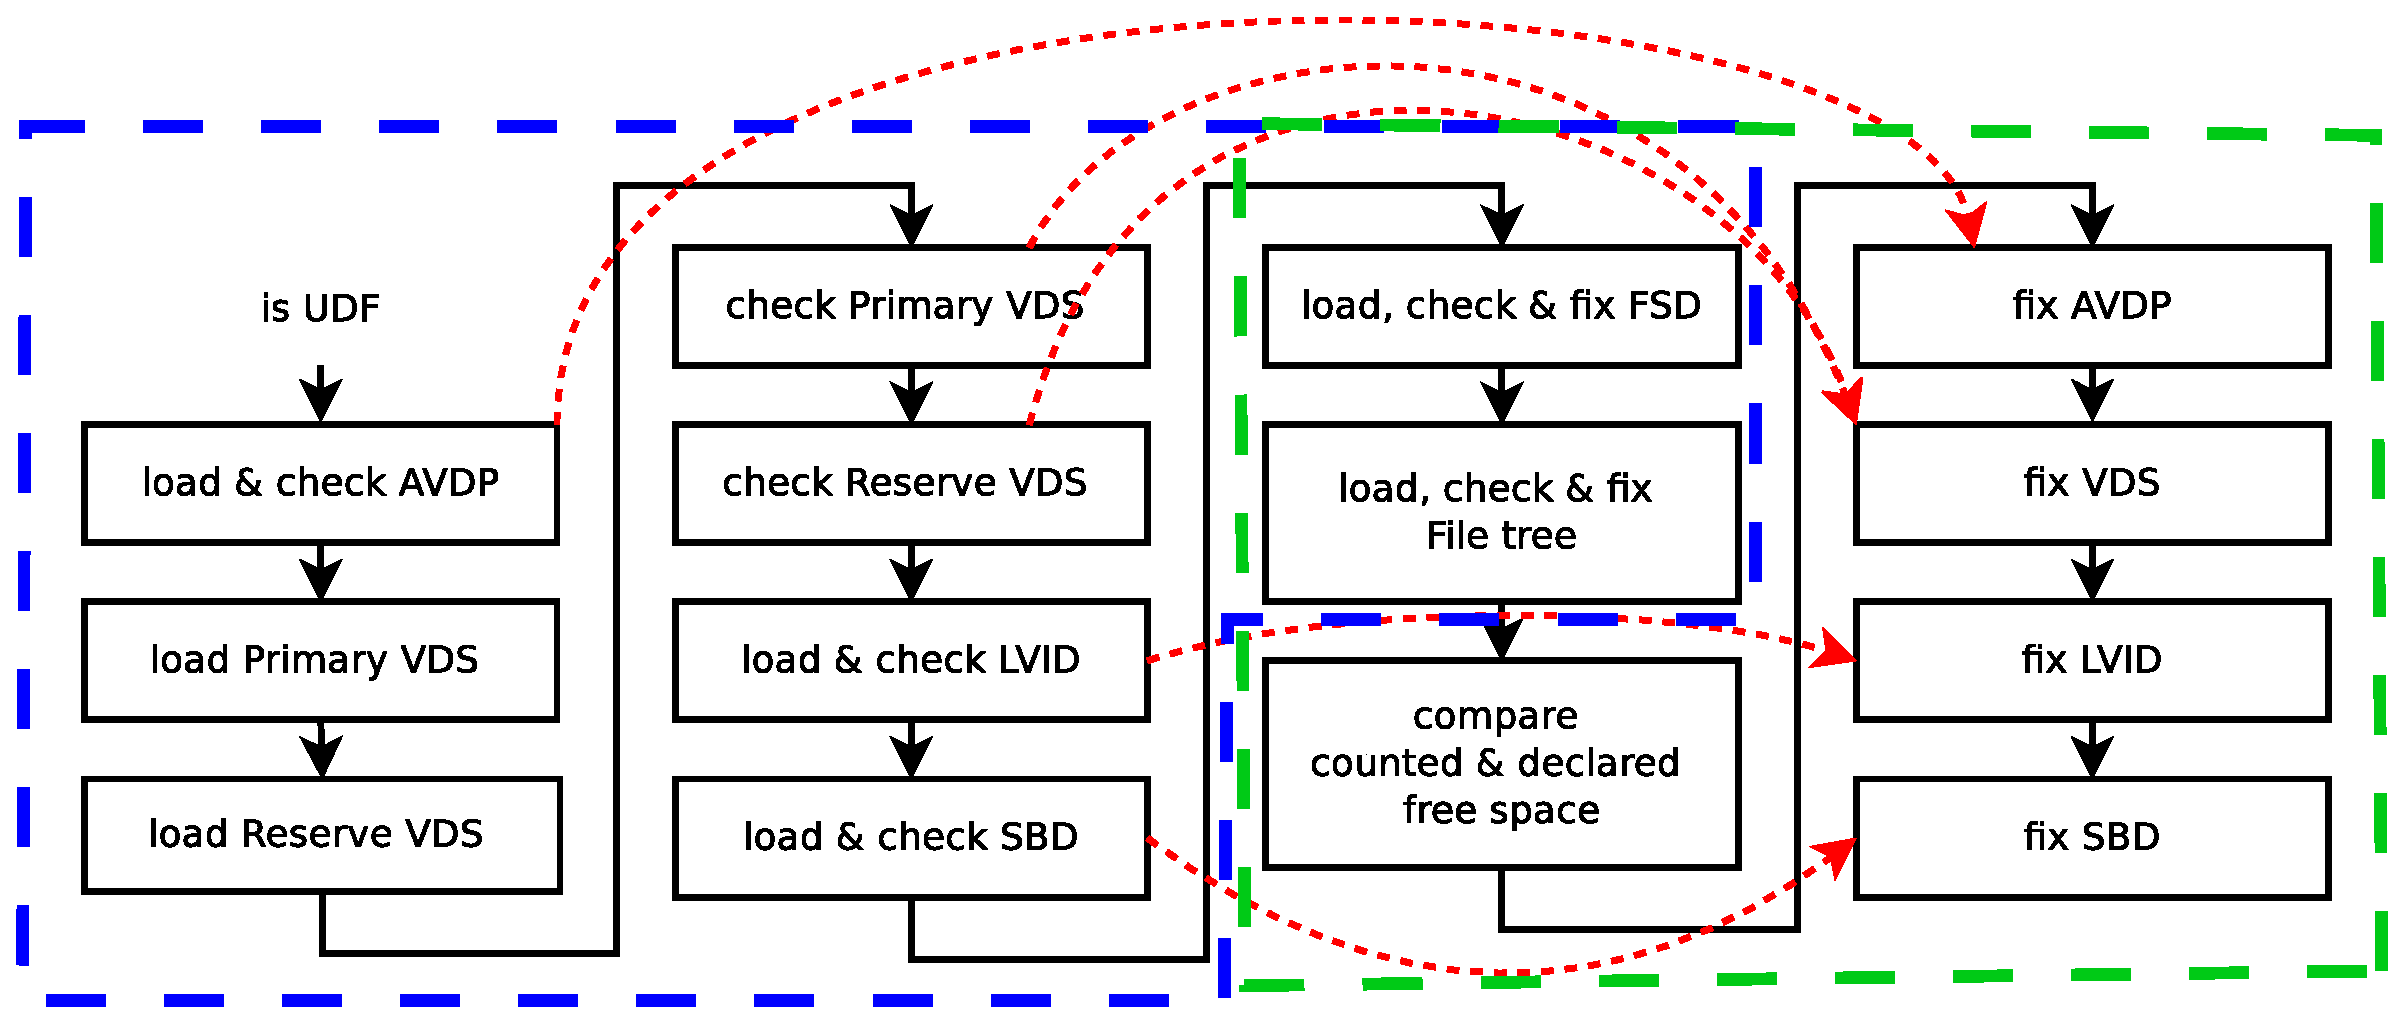
\includegraphics[scale=0.4]{obrazky/steps-korekce.eps}
    \caption{Zjednodušený algoritmus detekce a korekce}
    \label{fig:steps-korekce}
\end{figure}
V tomto obrázku, který navazuje na předchozí je cílem naznačit posloupnost jednotlivých operací a ukázat toky chybových stavů z detekcí ke korekcím (červené tečkované šipky). Modrý rámeček je část detekční, která je popsaná v předchozí části a zelený rámeček je část korekční. Jak je vidět, protínají se u práce s deskriptorem FSD a se souborovým stromem. Důvodem je předejití zbytečnému dvojímu procházení souborovým stromem. Proto jsou chyby v něm opravovány jak jsou nacházeny. Zbytek oprav již je ve svých oddělených krocích.

Důležitým detailem, který není v obrázku pro jednoduchost naznačen, je skutečnost, že každá korekce (t.j. zápis na médium) musí být autorizována uživatelem nebo apriori schválena při spuštění programu. Tudíž libovolná oprava může být přeskočena.

\section{Implementace nástroje pro detekci a korekci chyb}
\label{sec:implementace}
Implementace nástroje \texttt{udffsck} bude provedena v rámci balíčku \texttt{udftools}. Bude tak navazovat na existující sdílenou knihovnu, která obsahuje sdílené hlavičky s definicemi deskriptorů podle standardu ECMA-167.

Struktura nástroje bude rozdělena do třech částí. V první části bude probíhat načtení média a parsování vstupních parametrů. Druhá část bude detekovat přítomnost UDF, načítat deskriptory souborového systému a strom souborů a bude detekovat chyby v nich. Třetí část bude opravovat nalezené chyby na základě výsledků z předchozí části. Návrh jednotlivých částí je popsán v předchozí kapitole \ref{sec:navrh}.

Pokud rozebereme implementaci na menší části, dostaneme se již na úroveň jednotlivých kroků implementace. Ta bude postupovat podle algoritmu popsaném v předchozí kapitole, viz obrázek \ref{fig:steps-korekce}. Bude vytvořena struktura pro přenos chybové informace mezi detekčními a korekčními algoritmy, stejně tak strkuktura nesoucí pracovní informace o médiu. 

Nástroj bude vytvořen v jazyce C podle standardu C99 a bude využívat funkce poskytnuté prostředním GNU/Linux. Bude přeložitelný pomocí GCC pro ostré nasazení a pomocí LLVM CLANG pro vývoj. Důvodem je integrovaná funkce překladače LLVM CLANG \textit{Address Sanitizer}, který poskytuje užitečné informace o správě paměti, respektive při jejím porušení. Díky tomu je snažší odhalit neodalokovanou paměť, přetečení mezi paměťovými oblastmi a v případě havárie programu vypíše užitečné informace kde v paměti k chybě došlo včetně zásobníku volání funkcí které k tomu vedlo. Dále potřeba použít debugger, zde bude použit GDB. K vytvoření testů bude použita knihovna CMocka 1.1.0, ve které vzniknou v první řadě provozní testy celého programu, případně může být použita k tvorbě Unit Testů. Dokumentace k programu bude vytvořena pomocí nástroje Doxygen, který je určený k automatickému generování přehledné dokumentace z komentářů ve zdrojových kódech. Jako editor bude použitý Vim.

Vzhledem k závislostem zbytku balíčku (hlavně sdílené knihovny) je k překladu potřeba použít GNU Autotools spolu s knihovnou LibTool a Readline, která závisí na knihovně Ncurses. Tímto by měly být splněny požadavky pro implementaci.

Nástroj bude nutné testovat během vývoje vůči různým vzorkům souborových systémů UDF. K jejich vytvoření bude použit přednostně nástroj \texttt{mkudffs} z balíčku \texttt{udftools}, v menšině případů obrazy disků vytvořené na platformě Microsoft Windows a Apple macOS. Tyto obrazy disků budou následně poškozovány ať už cíleným přepisováním částí obrazů s cílem poškodit konkrétní části nebo budou nahrány nástrojem \texttt{dd} na flash disk a budou poškozovány odpojením disku během operace s médiem.

Závěrem implementační fáze bude začlenění výsledného \texttt{udffsck} zpět do balíčku \texttt{udftools}, ze kterého je rozvětven. Tento krok předpokládá funkční a otestovaný nástroj s vytvořenou manuálovou stránkou. K tomu, pro budoucí udržovatelnost, je nutné přiložit skupinu testů, které mohou probíhat automaticky bez účasti vývojáře a vracejí binární výsledek pokud test uspěl nebo selhal. Více o publikaci nástroje je v kapitole \ref{ch:publikace}.

Jednotlivé části implementace jsou detailněji popsány v následujících podkapitolách.

\section{Realizace detekce chyb v deskriptoru}
\label{sec:realizace-detekce}
Detekce chyb v deskriptorech je implementována na úrovni porovnání kontrolních součtů a CRC. Další mechanismus, který je využíván, je ověření deklarovaného umístění deskriptoru vůči skutečnosti.

Kontrolní součty jsou implementovány mou funkcí

\centerline{\texttt{\detokenize{uint8_t calculate_checksum(descTag tag)}}}

v souboru \texttt{udffsck.c}. Tato funkce pouze počítá kontrolní součet (viz. kapitola \ref{subsec:checksum}) nad zadaným tagem a výsledek výpočtu je vrácen jako návratová hodnota. Proto je zapouzdřena do funkce
 
\centerline{\texttt{\detokenize{int checksum(descTag tag)}}}

která přidává porovnání s referenční hodnotou kontrolního součtu, který je uložen v tagu. Takto fukce vrací 0 při rozdílu a nenulovou hodnotu při shodě.

CRC je počítáno funkcí sdílené knihovny, která je součástí balíku. Ta byla opět zapouzdřena funkcí

\centerline{\texttt{\detokenize{int crc(void * desc, uint16_t size)}}}

aby vracela tentokrát 0 při neshodě a nenulovou hodnotu při shodě. Oproti funkci pro výpočet kontrolního součtu je třeba funkci pro výpočet CRC dodat i délku. Důvodem tohoto oproti výpočetu kontrolního součtu pro \textit{DescriptorTag} je, že \textit{tag} má fixní délku a tu lze zjistit ze struktury, která jej popisuje pomocí funkce \texttt{sizeof()}. Deskriptory ovšem tuto vlastnost nemají. Jsou deskriptory, které mají délku fixní, ale část má délku proměnnou podle dat, která nesou (například délka struktury \textit{File Entry} je závislá na tom, jestli se jedná o soubor nebo adresář a v případě adresáře ještě kolik dalších deskriptorů je uvnitř.) Stejně tak není možné počítat nad celou délkou sektoru, protože CRC se liší podle délky, i když je zbytek vstupní sekvence složen pouze z nulových hodnot. Více o tomto je popsáno v kapitole \ref{subsec:crc}.

\section{Oprava deskriptoru}
\label{sec:oprava-deskriptoru}
Oprava deskriptoru při detekci chyby pomocí kontrolních mechanismů CRC, kontrolní součet nebo špatné pozice v \textit{Tag Location} probíhá v šesti krocích. Předpokladem takové opravy je existence správného zdrojového deskriptoru nebo dostatek dat pro jeho znovuvytvoření. Kroky opravy jsou tyto:
\begin{enumerate}
    \item Určení pozic zdrojového (správného) deskriptoru a cílového (defektního) deskriptoru.
    \item Zkopírování zdrojového deskriptoru do paměti. Tímto vytvoříme nový cílový deskriptor.
    \item Opravení položky \textit{Tag Location} v tagu nového cílového deskriptoru podle pozice původního cílového deskriptoru.
    \item Výpočet CRC nad novým cílovým deskriptorem a uložení výsledku do tagu. (Teoreticky nadbytečný krok, CRC by mělo být stejné jako u původního deskriptoru. Tento krok je užitečný pro vývoj kdy lze tímto oveřit, že byl zkorpírovaný celý zdrojový deskriptor.)
    \item Výpočet kontrolního součtu tagu nového cílového deskriptoru a uložení výsledku do tagu. (Zde již je nutné kontrolní součet spočítat, protože se změnila pozice uložená v tagu podle nového umístění deskriptoru.)
    \item Zkopírování nového cílového deskriptoru na místo původního cílového deskriptoru.
\end{enumerate}

\section{Mapa chyb}
\label{sec:mapa-chyb}
Účelem takzvané mapy chyb (neboli struktury \texttt{\detokenize{vds_sequence_t}}) je zapouzdření chyb, které jsou detekovány napříč médiem v deskriptorech, vyjma chyb v deskriptorech dat. Její struktura je v tabulce \ref{tab:err-seq}.

Jak je vidět, je složena z malých struktur s názvem \texttt{\detokenize{metadata_t}}. Ty jsou popsány tabulkou \ref{tab:metadata-t}. Jak je vidět, obsahuje pouze identifikátor deskriptoru (použité pouze u VDS, více v kapitole \ref{sec:nacteni-a-oprava-vds}), pozici deskriptoru a bitové pole chyb. Význam jednotlivých bitů je popsán v tabulce \ref{tab:E-codes}.
\begin{table}[hb]
    \begin{tabular}{ | l | l | p{2.3cm} | p{3.6cm} | p{5.5cm} | }
        \hline
        Adresa  & Délka [B]   & Jméno položky & Datový typ & Popis \\ \hline\hline
        0       & 21          & anchor         & pole \detokenize{metadata_t} \ref{tab:metadata-t} & Chyby v AVDP \\ \hline 
        21      & 56          & main           & pole \detokenize{metadata_t} \ref{tab:metadata-t} & Chyby v Hlavním VDS \\ \hline 
        77      & 56          & reserve        & pole \detokenize{metadata_t} \ref{tab:metadata-t} & Chyby v Záložním VDS \\ \hline 
        133     & 7           & lvid           & \detokenize{metadata_t} \ref{tab:metadata-t} & Chyby v LVID \\ \hline 
        140     & 7           & pd             & \detokenize{metadata_t} \ref{tab:metadata-t} & Chyby v SBD (referencováno z PD) \\ \hline 
    \end{tabular}
    \caption{Formát struktury \texttt{vds\_sequence\_t} (Mapa chyb)\label{tab:err-seq}}
\end{table}
\begin{table}[hb]
    \begin{tabular}{ | l | l | p{2.3cm} | p{3.6cm} | p{5.5cm} | }
        \hline
        Adresa  & Délka [B]   & Jméno položky & Datový typ & Popis \\ \hline\hline
        0       & 2          & tagIdent       & Uint16     & Identifikátor deskriptoru \\ \hline 
        2       & 4          & tagLocation    & Uint32     & Pozice deskriptoru \\ \hline 
        6       & 1          & error          & Uint8      & Bitové pole nalezených chyb (tabulka \ref{tab:E-codes}) \\ \hline 
    \end{tabular}
    \caption{Formát struktury \texttt{metadata\_t}\label{tab:metadata-t}}
\end{table}
\begin{table}
    \begin{tabular}{ | l | l | l | }
        \hline
        Název & Maska & Význam \\ \hline\hline
        \texttt{E\_CHECKSUM} & \texttt{0b00000001} & Chyba v konrolním součtu \\ \hline
        \texttt{E\_CRC}      & \texttt{0b00000010} & Chyba v CRC \\ \hline
        \texttt{E\_POSITION} & \texttt{0b00000100} & Chyba v umístění deskriptoru\\ \hline
        \texttt{E\_WRONGDESC}& \texttt{0b00001000} & Nenalezen očekávaný deskriptor (použito pouze pro AVDP)\\ \hline
        \texttt{E\_UUID}     & \texttt{0b00010000} & Chyba UUID souboru \\ \hline
        \texttt{E\_TIMESTAMP}& \texttt{0b00100000} & Chyba časové značky souboru\\ \hline
        \texttt{E\_FREESPACE}& \texttt{0b01000000} & Chyba v objemu volného místa\\ \hline
        \texttt{E\_FILES}    & \texttt{0b10000000} & Lišící se počet souborů nebo složek\\ \hline
    \end{tabular}
    \caption{Chybové kódy pro strukturu \texttt{metadata\_t}\label{tab:E-codes}}
\end{table}

\section{Výstup a ovládání nástroje}
Nástroj \texttt{udffsck} je navržen po vzoru ostatních nástrojů z rodiny \texttt{fsck}. Tomu bude odpovídat i jeho ovládání a výstup.

Vstupy různých \texttt{fsck} nástrojů se liší podle jednotlivých souborových systémů, ale kvůli zapouzdřitelnosti musí dodržovat návratové hodnoty pro různé druhy chyb. Jedná se o tyto hodnoty:
\begin{itemize}
    \item 0 - Bez chyb 
    \item 1 - Opraveny chyby na souborovém systému
    \item 2 - Opraveny chyby na souborovém systému, doporučený reboot (nepodporováno) 
    \item 4 - Chyby souborového systému zůstaly neopraveny
    \item 8 - Chyba programu
    \item 16 - Chybné vstupní parametry
    \item 32 - Kontrola byla přerušena na základě uživatelského požadavku
    \item 128 - Chyba sdílené knihovny (nepodporováno)
\end{itemize}
Návratová hodnota je součtem těchto hodnot v případě souběhu.

Má implementace převzala tuto skladbu návratových hodnot s výjimkou kódů 2 a 128, které nejsou v tuto chvíli podporovány.

Protože se jedná o terminálový program, není obsaženo žádné grafické uživatelské rozhraní. Nástroj vypisuje informativní hlášení na standardní výstup \texttt{stdout} a chybová hlášení na chybový výstup \texttt{stderr}. Pokud je vyžadována interakce s uživatelem, jeho reakce je převzata ze standardního vstupu \texttt{stdin}.

Struktura volání nástroje \texttt{udffsck} je toto:

\centerline{\texttt{udffsck [-vvvciph] [-B BLOCKSIZE] medium}}

Jak je vidět, nástroj implementuje několik přepínačů a jeden vstupní parametr. Dále požaduje cestu k médiu, které má být kontrolováno (argument  \texttt{medium}). 
Rozbor vstupních paramtrů je tento:
\begin{itemize} 
    \item \texttt{-B BLOCKSIZE} - Vnucení velikosti bloku místo autodetekce.
    \item \texttt{-c} - Médium bude pouze zkontrolováno, žádné chyby nebudou opraveny. Výchozí chování, pokud je nástroj zavolán bez přepínačů.
    \item \texttt{-i} - Interaktivní oprava za účasti uživatele. Při použití tohoto přepínače je před každou opravou požadována autorizace od uživatele. 
    \item \texttt{-p} - Automatická oprava média. Výsledek této opravy je stejný jako kdyby uživatel v interaktivním režimu odpověděl na všechny otázky Ano.
    \item \texttt{-h} - Stručná nápověda k programu
    \item \texttt{-v} - Zvýšená úroveň výpisů do terminálu na hladinu \textit{Warning}. K chybovým hlášením (které nelze potlačit) se přidají i varovná hlášení.
    \item \texttt{-vv} - Zvýšení úrovně hlášení na hladinu zpráv. Bude vypisováno to co na \texttt{-v} a k tomu pracovní zprávy. Vhodné pro uživatele.
    \item \texttt{-vvv} - Zvýšení úrovně hlášení na hladinu ladění. Bude vypisováno to co ne \texttt{-vv} a k tomu ladicí hlášení. Vhodné pro vývojáře.
\end{itemize}
Ukázkové volání nástroje může vypadat například takto:

\centerline{\texttt{udffsck -vvc -B 2048 /dev/sdb1}}

Stejné informace budou dostupné i s distribucí nástroje a to v manuálové stránce, kterou jsem napsal k \texttt{udffsck}. Její přepis je v příloze \ref{ch:manpage}.
Ukázkový výstup programu je v příloze \ref{lst:bs512} včetně komentáře jednotlivých částí výstupu. 

\section{Načtení média a jeho příprava na zpracování}
Životní cyklus média v mé implementaci začíná předáním cesty k médiu při spuštění programu. Ta musí vést přímo k zařízení jako takovému, nikoli k místu, kam je připojeno.

Médium je na základě cesty načteno. Jednou pomocí funkce \texttt{open(2)} \cite{man-open} pro práci samotnou, podruhé pomocí \texttt{fopen(3)} \cite{man-fopen} pro nalezení velikosti média. Volání \texttt{fopen(3)} je pouze pro čtení, protože po úspěšném zjištění velikosti média není dále potřeba. Volání \texttt{open(2)} se liší podle dalších argumentů při spuštění programu. Pokud je médium pouze kontrolováno, je otevřeno pro čtení. Pokud je požadována i korekce (ať už automatická nebo interaktivní), je otevřeno pro čtení a zápis.

Dalším krokem po načtení je zamčení média pomocí funkce \texttt{flock(2)} \cite{man-flock}. Důvodem je zamezení paralelního přístupu k médiu při kontrole. Není žádoucí, aby médium mohlo být měněno během kontroly a korekce. Použití této funkce je implementováno jako neblokující. V případě nemožnosti uzamčít médium program skončí s chybou.

Po úspěšném zamčení média následuje namapování média do paměti funkcí \texttt{mmap(2)} \cite{man-mmap}. Ta přebírá referenci na médium z funkce \texttt{open(2)} a stejně tak se liší její parametry podle požadavků na kontrolu nebo i korekci. Pokud je médium úspěšně namapováno do paměti, je možné přistoupit k práci s médiem jako takovým.

První otázka, která vyvstává, je duální otevření stejného souboru pouze pro zjištění velikosti média. Existuje funkce \texttt{fstat(2)} \cite{man-fstat}, která slouží ke zjištění údajů o souboru a pracuje s referencí z volání \texttt{open(2)}. Tato funkce naplní strukturu \texttt{struct stat} a ta obsahuje údaje jako je velikost souboru nebo ideální velikost bloku. Problém je, že tato funkce selže při použití se surovým médiem (tímto je myšlen přístup přímo na úložiště přes cestu \texttt{/dev/sdX}). Pokud by program pracoval pouze s obrazy disků, které jsou uložené jako soubor na souborovém systému, použití této funkce by bylo ideální. Ovšem v tomto případě je nejpřijatelnější přístup načtení média znovu a použití funkce \texttt{fseeko(3)} \cite{man-fseeko} s parametrem \texttt{SEEK\_END} a následně zjištění aktuální pozice funkcí \texttt{ftello(3)} \cite{man-ftello}. Důvodem použití \texttt{fseeko(3)} a \texttt{ftello(3)} místo \texttt{fseek(3)} \cite{man-fseek} a \texttt{ftell(3)} \cite{man-ftell} je návratový typ \texttt{off\_t}, který na rozdíl od \texttt{long} neumožňuje záporné hodnoty, tudíž je použití těchto funkcí preferované v nových projektech.

Druhá otázka vyvstává u použití funkce \texttt{mmap(2)} a výhodám oproti funkcím \texttt{read(2)} \cite{man-read} a \texttt{write(2)} \cite{man-write}. Důvodů je několik, počínaje pohodlností použití. Pokud je soubor mapovanán do paměti, je s ním z hlediska programu pracováno jako s jednorozměrným polem o velikosti mapovaného souboru. Tím pádem lze přistupovat na libovolné místo souboru bez nutnosti používat \texttt{lseek(2)}, lze snadno referencovat kusy souboru do struktur a poté s ním pracovat ve struktuře místo nutnosti ho do struktury kopírovat. Rizikem tohoto přístupu je setření hranice mezi médiem a operační pamětí a tudíž opatrnost při zápisu zpět do média, aby nedošlo k nežádoucí modifikaci souboru.

\section{Kontrola přítomnosti identifikátoru souborového systému UDF}
\label{sec:kontrola-pritomonosti-udf}
Po úspěšném načtení média je prvním krokem před jakoukoli další prací kontrola přítomnosti správného souborového systému, v tomto případě UDF. Tato kontrola probíhá kontrolou oblasti \textit{Volume Recogniton Sequence} (VRS) pomocí funkce \texttt{is\_udf()}. Tato funkce načte blok na sektoru 16. Tento blok je fixní místo na souborovém systému a je shodný pro UDF a ISO~9660, který je přímý předchůdce UDF. Zvláštností načítání VRS je velikost sektoru. Z důvodu zachování kompatibility s ISO~9660, který podporuje pouze velikost bloku 2048~B, je tato velikost převzata jako konstanta, nezávisle na skutečné velikosti bloku média. Ovšem i tento axiom má výjimku a to že toto platí pouze do velikosti bloku 2048~B. Na médiích s větší velikostí bloku je již použita skutečná velikost bloku místo 2048~B. To je možné díky skutečnosti, že ISO~9660 nikdy nebude možné použít na takovém médiu. U médií s menší velikostí bloku by ISO~9660 stále použít šlo, stačí pouze zapisovat na více bloků místo jednoho při zápisu 2048~B.

Kontrola samotná probíhá načtením struktur VRS, kde se vyhledávají deskriptory popisující UDF, t.j. deskriptory obsahující identifikátor \texttt{NSR01}, \texttt{NSR02} nebo \texttt{NSR03}. Pokud je takovýto identifikátor nalezen, a spolu s ním je i nalezen identifikátor \texttt{TEA01} (\textit{Terminating Extended Area}), je médium prohlášeno za správné a může se přistoupit ke kontrole. Pokud je nalezena identifikace UDF ale ne kompletní \textit{Extended Area}, může to znamenat neuzavřené médium a to pro další kontrolu znamená jiné umístění AVDP. Kontrola je ale možná. Pokud nebyl nalezen identifikátor UDF, kontrola končí chybou a program končí, protože nebylo možné detekovat přítomnost UDF.

Druhou činností, kterou funkce \texttt{is\_udf()}, pokrývá je první pokus o detekci velikosti sektoru. Ta postupně zkouší načíst platné deskriptory pro různé povolené velikosti sektoru (hodnoty dělitelné beze zbytku 512, v praxi ovšem pouze omezená řada 512, 1024, 2048, 4096~B) a ukládá hodnotu, kdy se to podaří. Prakticky by se to mělo podařit pouze pro velikost sektoru 2048~B a 4096~B. Pro velikosti sektoru média 2048~B včetně je obvykle detekovaná velikost sektoru 512~B (neboli nejnižší možná). S touto hodnotou poté dále pracuje detekce AVDP, která ji používá jako výchozí bodu svého hledání velikosti sektoru.

\section{Načtení, kontrola a korekce deskriptoru AVDP}
\label{sec:nacteni-a-oprava-avdp}
\textit{Anchor Volume Descriptor Pointer} (AVDP) je klíčovou částí UDF, protože určuje výchozí bod pro čtení souborového systému (na rozdíl od VRS, které pouze určuje přítomnost UDF). Jak je uvedeno v kapitole \ref{subsec:avdp}, UDF rozlišuje čtyři možná umístění AVDP, přičemž přítomné na mediu může být jedno nebo až tři.

Jejich načítání pro potřeby další práce se souborovým systém lze popsat algoritmem na obrázku \ref{fig:avdp}. Algoritmus prochází možné lokace AVDP, dokud neuspěje nebo nedojdou možnosti. Pro potřeby kontroly a opravy média je třeba po nalezení alespoň jednoho správného AVDP ostatní podle něj opravit.

Jak je uvedeno, je možné, aby bylo na médiu AVDP uloženo jednou nebo až třikrát. Toto souvisí se stavem finalizace média. Více o finalizaci je v kapitole \ref{sec:udf-struktura}.

Z toho vyplývá, že oprava AVDP je možná pouze na uzavřených médiích. Důvodem je požadavek opravného algoritmu na přítomnost alespoň jednoho nepoškozeného (správného) deskriptoru, který bude použit jako vzor pro opravu. Otevřená (neukončená) média mají pouze jeden AVDP, proto v případě jeho poškození není oprava možná.

Jedinou variantou by v takovém případě bylo prohledávání média po sektorech a hledání VDS deskriptorů. Toto ovšem není v tuto chvíli implementováno.

Poté, co jsou nalezeny AVDP na svých pozicích (t.j. sektoru 256 a na posledním sektoru, případně na sektoru 512) a je určeno, který z nich je poškozený a který je v pořádku, lze přistoupit k opravě, pokud je alespoň jeden v pořádku.

Samotný opravný algoritmus je popsán v kapitole \ref{sec:oprava-deskriptoru}.

Detekovatelnou a opravitelnou chybou je nedodržení specifikace UDF\cite{osta-udf-0201}, kapitola 2.2.3.1 s 2.2.3.2 týkající se rezervované délky pro VDS. Minimální délka této oblasti je 16 sektorů pro hlavní VDS a 16 sektorů pro záložní VDS. Pokud je tento konflikt nalezen, oprava spočívá v kontrole možnosti rozšíření a následné nastavení správné velikosti rezervovaného místa.

Případné nalezené chyby jsou uloženy do struktur popsaných v kapitole \ref{sec:mapa-chyb}. V tomto případě může dojít k chybám v kontrolním součtu, v CRC, poloze deskriptoru a nalezení platného \emph{jiného} deskriptoru na pozici vyhrazené pro AVDP.

\begin{figure}[ht] 
    \centering
    %\resizebox{0.5\textwidth}{!}{\input{obrazky/avdp.tex}}}
    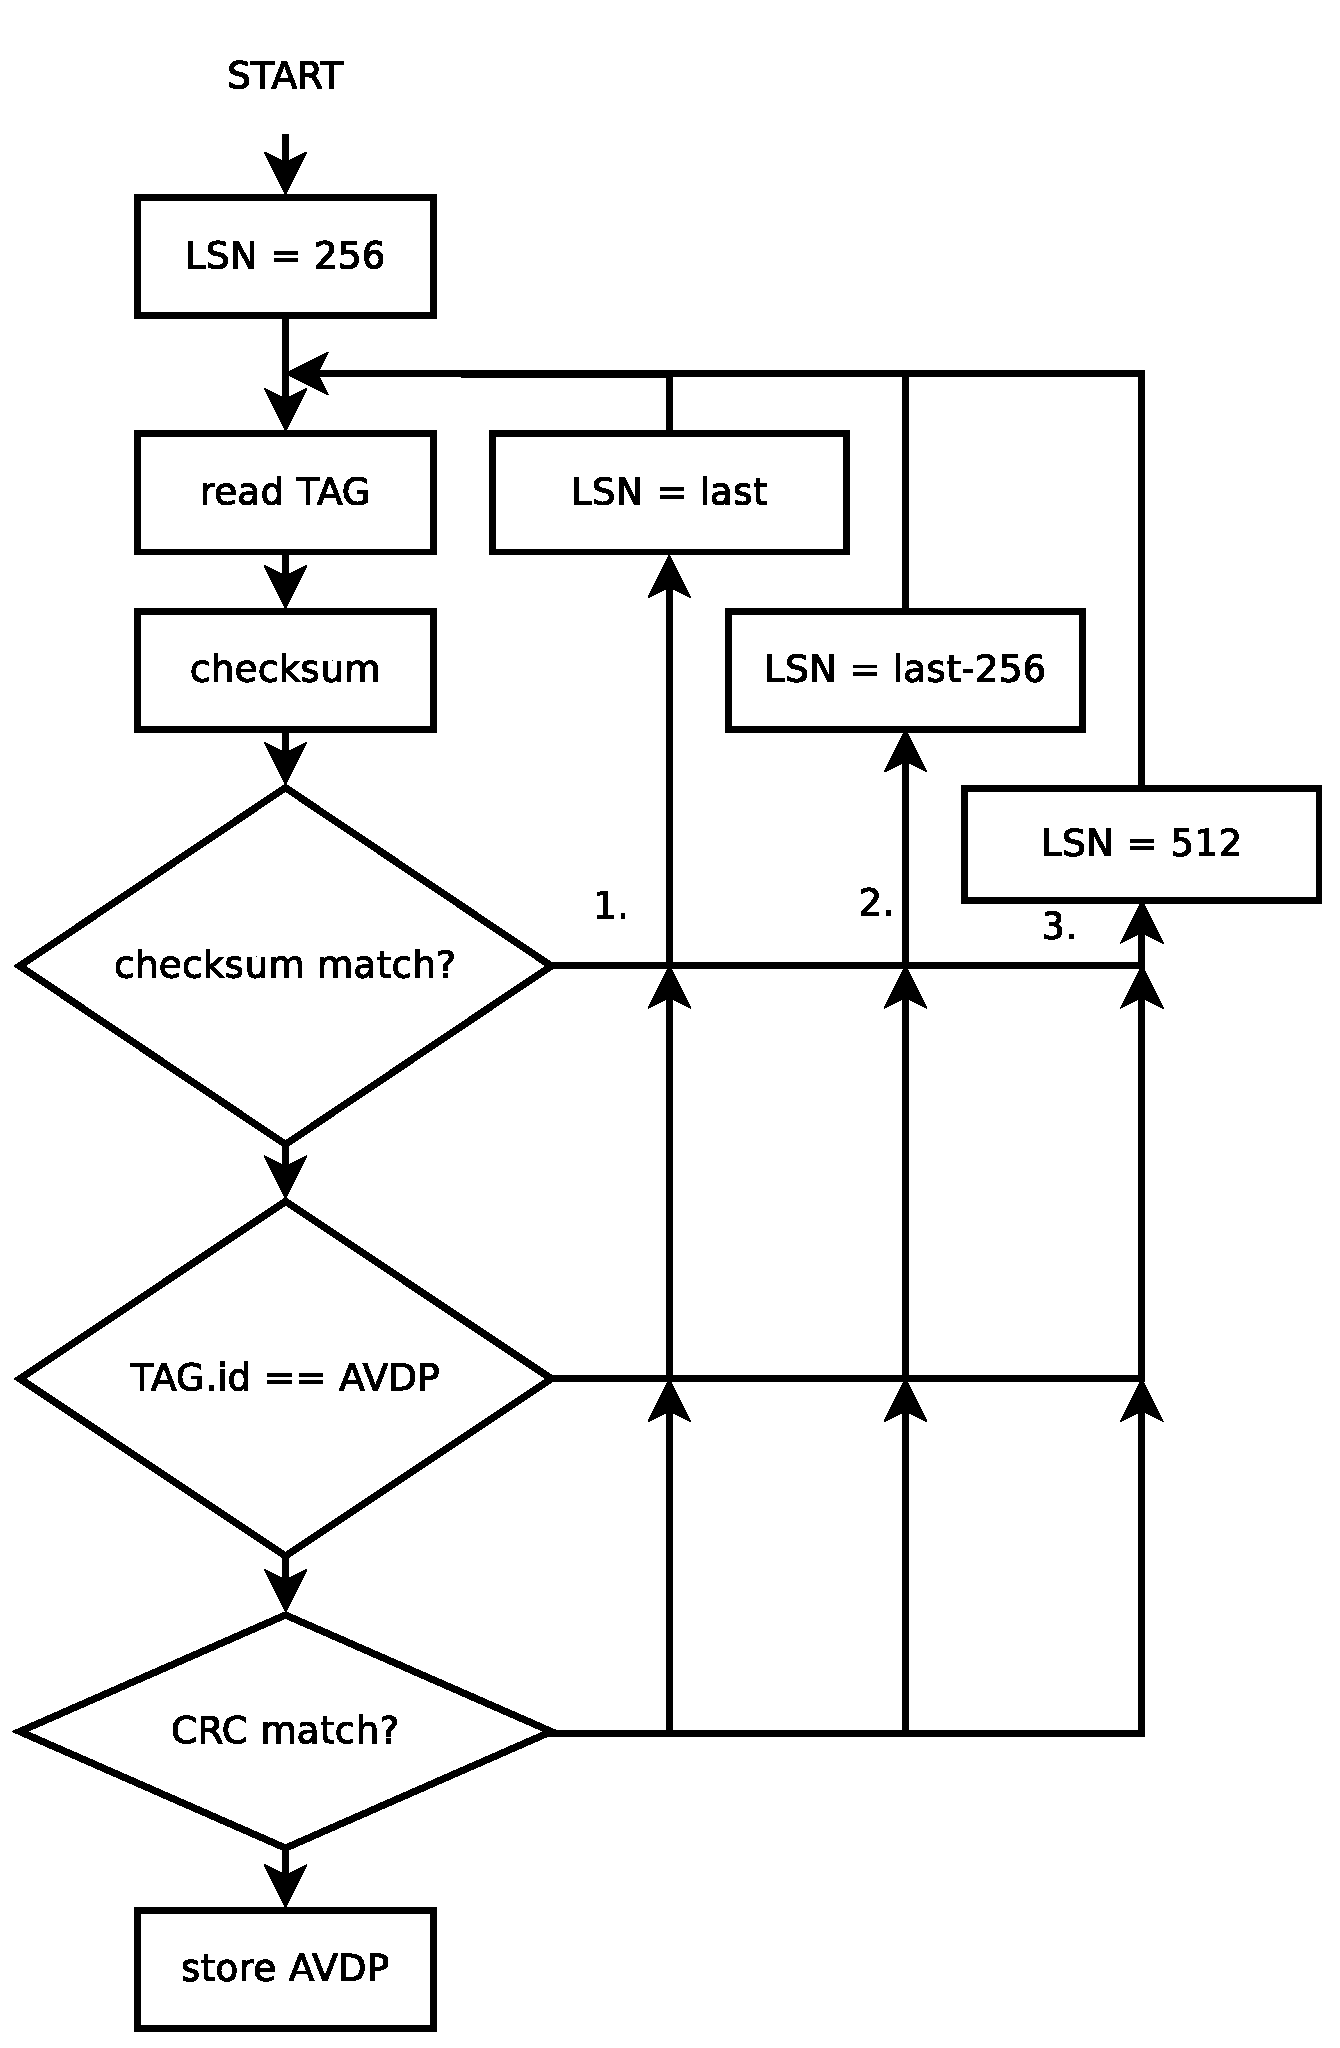
\includegraphics[scale=0.4]{obrazky/avdp.eps}
    \caption{Zjednodušený algoritmus načtení AVDP}
    \label{fig:avdp}
\end{figure}

\section{Načtení, kontrola a korekce deskriptoru VDS}
\label{sec:nacteni-a-oprava-vds}
Po úspěšném nalezení funkčního AVDP je možné načíst \textit{Volume Descriptor Sequence} (VDS). Tato skupina metadat je uložena na dvou místech, typicky jedno na začátku a druhé na konci média (ale není to pravidlem). Pozice obou je uložena právě v AVDP.

Tato skupina deskriptorů je popsána v kapitole \ref{subsec:vds}. Deskriptory jsou uloženy za sebou v jednotlivých sektorech, přičemž poslední musí být vždy \textit{Terminating Descriptor}. Jak hlavní, tak záložní VDS by měly být ekvivalentní (ačkoli ne nutně ve stejném pořadí.)

Jednotlivé deskriptory jsou načítány a ukládány do struktur pro další zpracování. První kontrola během načítání spočívá v porovnání kontrolního součtu tagu deskriptoru (viz kapitola \ref{sec:errordetection}). Pokud tato kontrola uspěje, je možné provést porovnání CRC, protože již máme díky ověřenému tagu jistou totožnost deskriptoru, jeho předpokládané CRC a polohu. Pokud kontrola CRC uspěje, zkontroluje se poloha deskriptoru vůči deklarovanému umístění v tagu. Pokud i tato kontrola je v pořádku, lze prohlásit tag za správný. Pokud by byl v pořádku jak kontrolní součet, tak CRC, ale bylo by špatně deklarované umístění, lze s tagem pracovat, protože data která nese, jsou s největší pravděpodobností v pořádku, ale je nutné opravit jeho umístění a následně přepočítat kontrolní součet a CRC. 
Oprava VDS je podobná jako oprava AVDP. Předpokladem úspěšné opravy je opět existence alespoň jednoho správného zdrojového deskriptoru od každého typu, který ve VDS je. Pokud je toto splněno, je oprava možná.

Algoritmus je navržen takto:
\begin{enumerate}
    \item Během načítání VDS (jak hlavního, tak záložního) je vytvářena mapa chyb na jednotlivých deskriptorech. Formát mapy je popsán v tabulce \ref{tab:err-seq}. 
    \item Na základě údajů mapy chyb je přistoupeno k opravě. Pokud je alespoň jeden z deskriptorů v pořádku, je použit algoritmus z kapitoly \ref{sec:oprava-deskriptoru}. Pokud ne, je vypsána chyba a pokračuje se k dalšímu deskriptoru.
    \item Krok 2 se opakuje, dokud není nalezen \textit{Terminating Descriptor}. Poté je oprava ukončena, protože byl nalezen konec VDS.
\end{enumerate}
Právě u korekce VDS může dojít k situaci, kdy bude část opravena a část nikoli. Dalším důležitým limitem je předpoklad, že jak hlavní, tak rezervní VDS mají stejné pořadí deskriptorů. Je to konvence, ovšem nikoli standard.

\section{Načtení, kontrola a korekce deskriptoru LVID}
\label{sec:nacteni-a-oprava-lvid}
\textit{Logical Volume Integrity Descriptor} (LVID) je důležitou částí UDF. Je umístěné mimo VDS a jeho pozice je uložena v LVD pod položkou \textit{Integrity Sequence Extent}. LVID není redundantní, což zjednodušuje práci s ním, ale zároveň se kvůli tomu jedná o slabé místo UDF. Ovšem je potřeba vzít v potaz skutečnost, že LVID lze v případě nepoškozeného souborového systému vytvořit znovu zpětně. V případě poškozeného souborového systému jej lze vytvořit též, ale s rizikem ztráty dat z důvodu nekompletní informace o souborovém systému v jiných deskriptorech.

Po kontrole kontrolního součtu a CRC je přistoupeno k samotnému načtení dat. Pro snažší práci s daty uloženými v LVID jsou vybraná data ukládána do struktury \texttt{filesystemStats}.

Protože nadřazeným standardem UDF je ECMA-167, je LVID popsáno podle ní. Ovšem samotnou implementací je UDF standard a ten využívá pole \textit{Implementation~Use}, kam ukládá tyto údaje:
\begin{itemize}
    \item Počet souborů na svazku
    \item Počet adresářů na svazku
    \item Minimální revize UDF, se kterou je možné médium číst
    \item Minimální revize UDF, se kterou je možné na médium zapisovat
    \item Maximální revize UDF, se kterou je možné na médium zapisovat
\end{itemize}
Podobná situace je u položky \textit{Logical Volume Contents Use}. UDF tuto položku používá k uložení \textit{Logical Volume Header Descriptor}, což je struktura popsaná pomocí standardu ECMA-167 s jediným cílem a tím je uložení \textit{Unique ID}, neboli unikátního identifikátoru, který nese každý soubor a adresář na médiu. Význam \textit{Unique ID} je popsán v kapitole \ref{sec:filetree}. LVID zde nese informaci o tom, jaké \textit{Unique ID} bude použito pro další záznam dat (což zároveň znamená, že toto \textit{Unique ID} musí být nejvyšší ze všech, co jsou uloženy na médiu.)

Další částí je \textit{Free Space Table}, což je tabulka obsahující informaci o velikosti logického svazku a volného místa na něm. Oba údaje jsou v logických blocích, nikoli v bytech.

Důležitou částí je i časová značka poslední modifikace logického svazku. Tato značka, uložená v UTC, by měla být vždy nejnovější ze všech časových značek na svazku.

Poslední položkou, která je důležitá pro prácí se svazkem, je \textit{Integrity Type}. Ten může být buď otevřený (\textit{Open}) nebo uzavřený (\textit{Close}). Princip otevřeného a uzavřeného média je popsán v kapitole \ref{sec:kontrolni-mechanismy}. Pokud je uzavřený, tak by měl být svazek v konzistentním stavu. Jestliže je otevřený, je možné, že probíhá zápisová operace, nebo že byl svazek během ní nesprávně odebrán. Tento indikátor pomáhá vyvolat požadavek na kontrolu média v operačním systému a pro kontrolu to je důležitý ukazatel upozorňující na pravděpodobnou nesrovnalost mezi deklarovaným volným místem a skutečností.
 
Korekce LVID je odlišná od ostatních korekcí z důvodu absence redundantního LVID. Z toho vyplývá, že LVID nelze v případě poškození opravit (t.j. pokud selže kontrolní součet nebo CRC.) LVID ale obsahuje důležité informace o konzistenci média (viz kapitola \ref{subsec:lvid}) a proto je korekce soustředěna na ně.

Opravují se tyto položky:
\begin{itemize}
    \item Vyvolání opravy SBD (kapitola \ref{sec:nacteni-a-oprava-sbd})
    \item Počet souborů a složek.
    \item Následující \textit{Unique ID}.
    \item Datum posledního záznamu se nastaví na čas opravy.
    \item Opraví se tabulka volného místa \textit{Free Space Table}.
    \item Médium se uzavře (\textit{Integrity type} se nastaví na \textit{Closed}).
    \item Přepočítá se kontrolní součet a CRC.
\end{itemize}
Korekce je spouštěna z několika různých důvodů, které sice ve většině případů nastávají současně, ale mohou se vyskytnout i odděleně. Jedná se o tyto zdroje:
\begin{itemize}
    \item Pokud bylo nalezeno \textit{Unique ID} stejné nebo větší jako uloženo v LVID.
    \item Pokud byl nalezen soubor s novějším datem, než je datum posledního záznamu v LVID.
    \item Pokud byla nalezena nesrovnalost v počtu souborů nebo složek uložených v LVID vůči skutečnému počtu.
    \item Pokud nekoresponduje objem volného místa s hodnotou deklarovanou v \textit{Free Space Table}.
    \item Pokud byl \textit{Integrity Type} ponechán ve stavu \textit{Open}.
\end{itemize}

\section{Načtení, kontrola a korekce deskriptoru SBD}
\label{sec:nacteni-a-oprava-sbd}
\textit{Space Bitmap Descriptor} je deskriptor popisující volné a obsazené místo na logickém svazku z hlediska umístění jednotlivých bloků. Jedná se o vektor bytů (\textit{Bitmap}) o délce $PocetLBN / 8$. Spolu s ním je uložena jeho délka (\textit{Number of Bytes}) a skutečný počet bloků (\textit{Number of Bits}). SBD je popsáno v kapitole \ref{subsec:pd-sbd}.
 
Každý jeden byte v tomto vektoru odpovídá osmi logickým blokům v přirozeném pořadí (nejméně významný bit odpovídá prvnímu bloku, nejvíce významný bit odpovídá osmému bloku).

Hodnota bitu označuje stav bloku. Logická 1 odpovídá volnému bloku, logická 0 obsazenému bloku. Přebývající bity v posledním bytu se označují jako obsazené.

Korekce probíhá tak, že během průchodu souborovým stromem (kapitola \ref{sec:filetree}) se vytváří nový vektor obsazeného místa o stejné velikosti jako původní. Ten slouží jako referenční mapa, která bude nakopírována na místo původní v případě nutnosti opravy.

Oprava je vyvolána automaticky při opravě LVID (kapitola \ref{sec:nacteni-a-oprava-lvid}), při rozdílu počtu použitých bloků oproti počtu ve vektoru \textit{Bitmap} nebo pokud při načítání došlo k chybě v kontrolním součtu nebo CRC.

Nutno podotknout, že SBD nemusí být vůbec na médiu přítomno. Jeho určením je totiž přednostně optimalizace zápisů u \textit{Rewritable} médií z hlediska přepisu jednou zapsaných sektorů. To ovšem nedává smysl pro \textit{Write Once} a \textit{Read Only} média, proto je tento deskriptor u nich vynechán.

\section{Kontrola a obnova stromu souborů}
\label{sec:filetree}
Obnova stromu uživatelských dat je klíčová část programu. Bez ní nemá tento nástroj význam. Vzhledem k faktu, že \texttt{fsck} nemá za cíl detekovat chyby v datech samotných a UDF také neimplementuje ochranné algoritmy na data samotná ale jen na metadata, není bohužel možné poškozená data ani detekovat a tudíž ani opravit. Je možné se pokusit zrekonstruovat adresářovou strukturu a určit místo, kde by data měla být.

Důvodem vynechání dat z detekce a korekce na úrovni \texttt{fsck} je skutečnost, že fyzické médium má integrované ochranné mechanismy v sobě, například v podobě ECC bloků. Proto se předpokládá, že pokud jsou data jednou korektně uložena, médium se postará o jejich správnost.

Ústředními deskriptory u stromu souborů jsou deskriptory \textit{(Extended) File Entry} (FE/EFE), který je popsaný v kapitole \ref{subsec:fe} a \textit{File Identifier Descriptor} (FID), který je popsaný v kapitole \ref{subsec:fid}.
 
\begin{figure}[!b] 
    \centering
    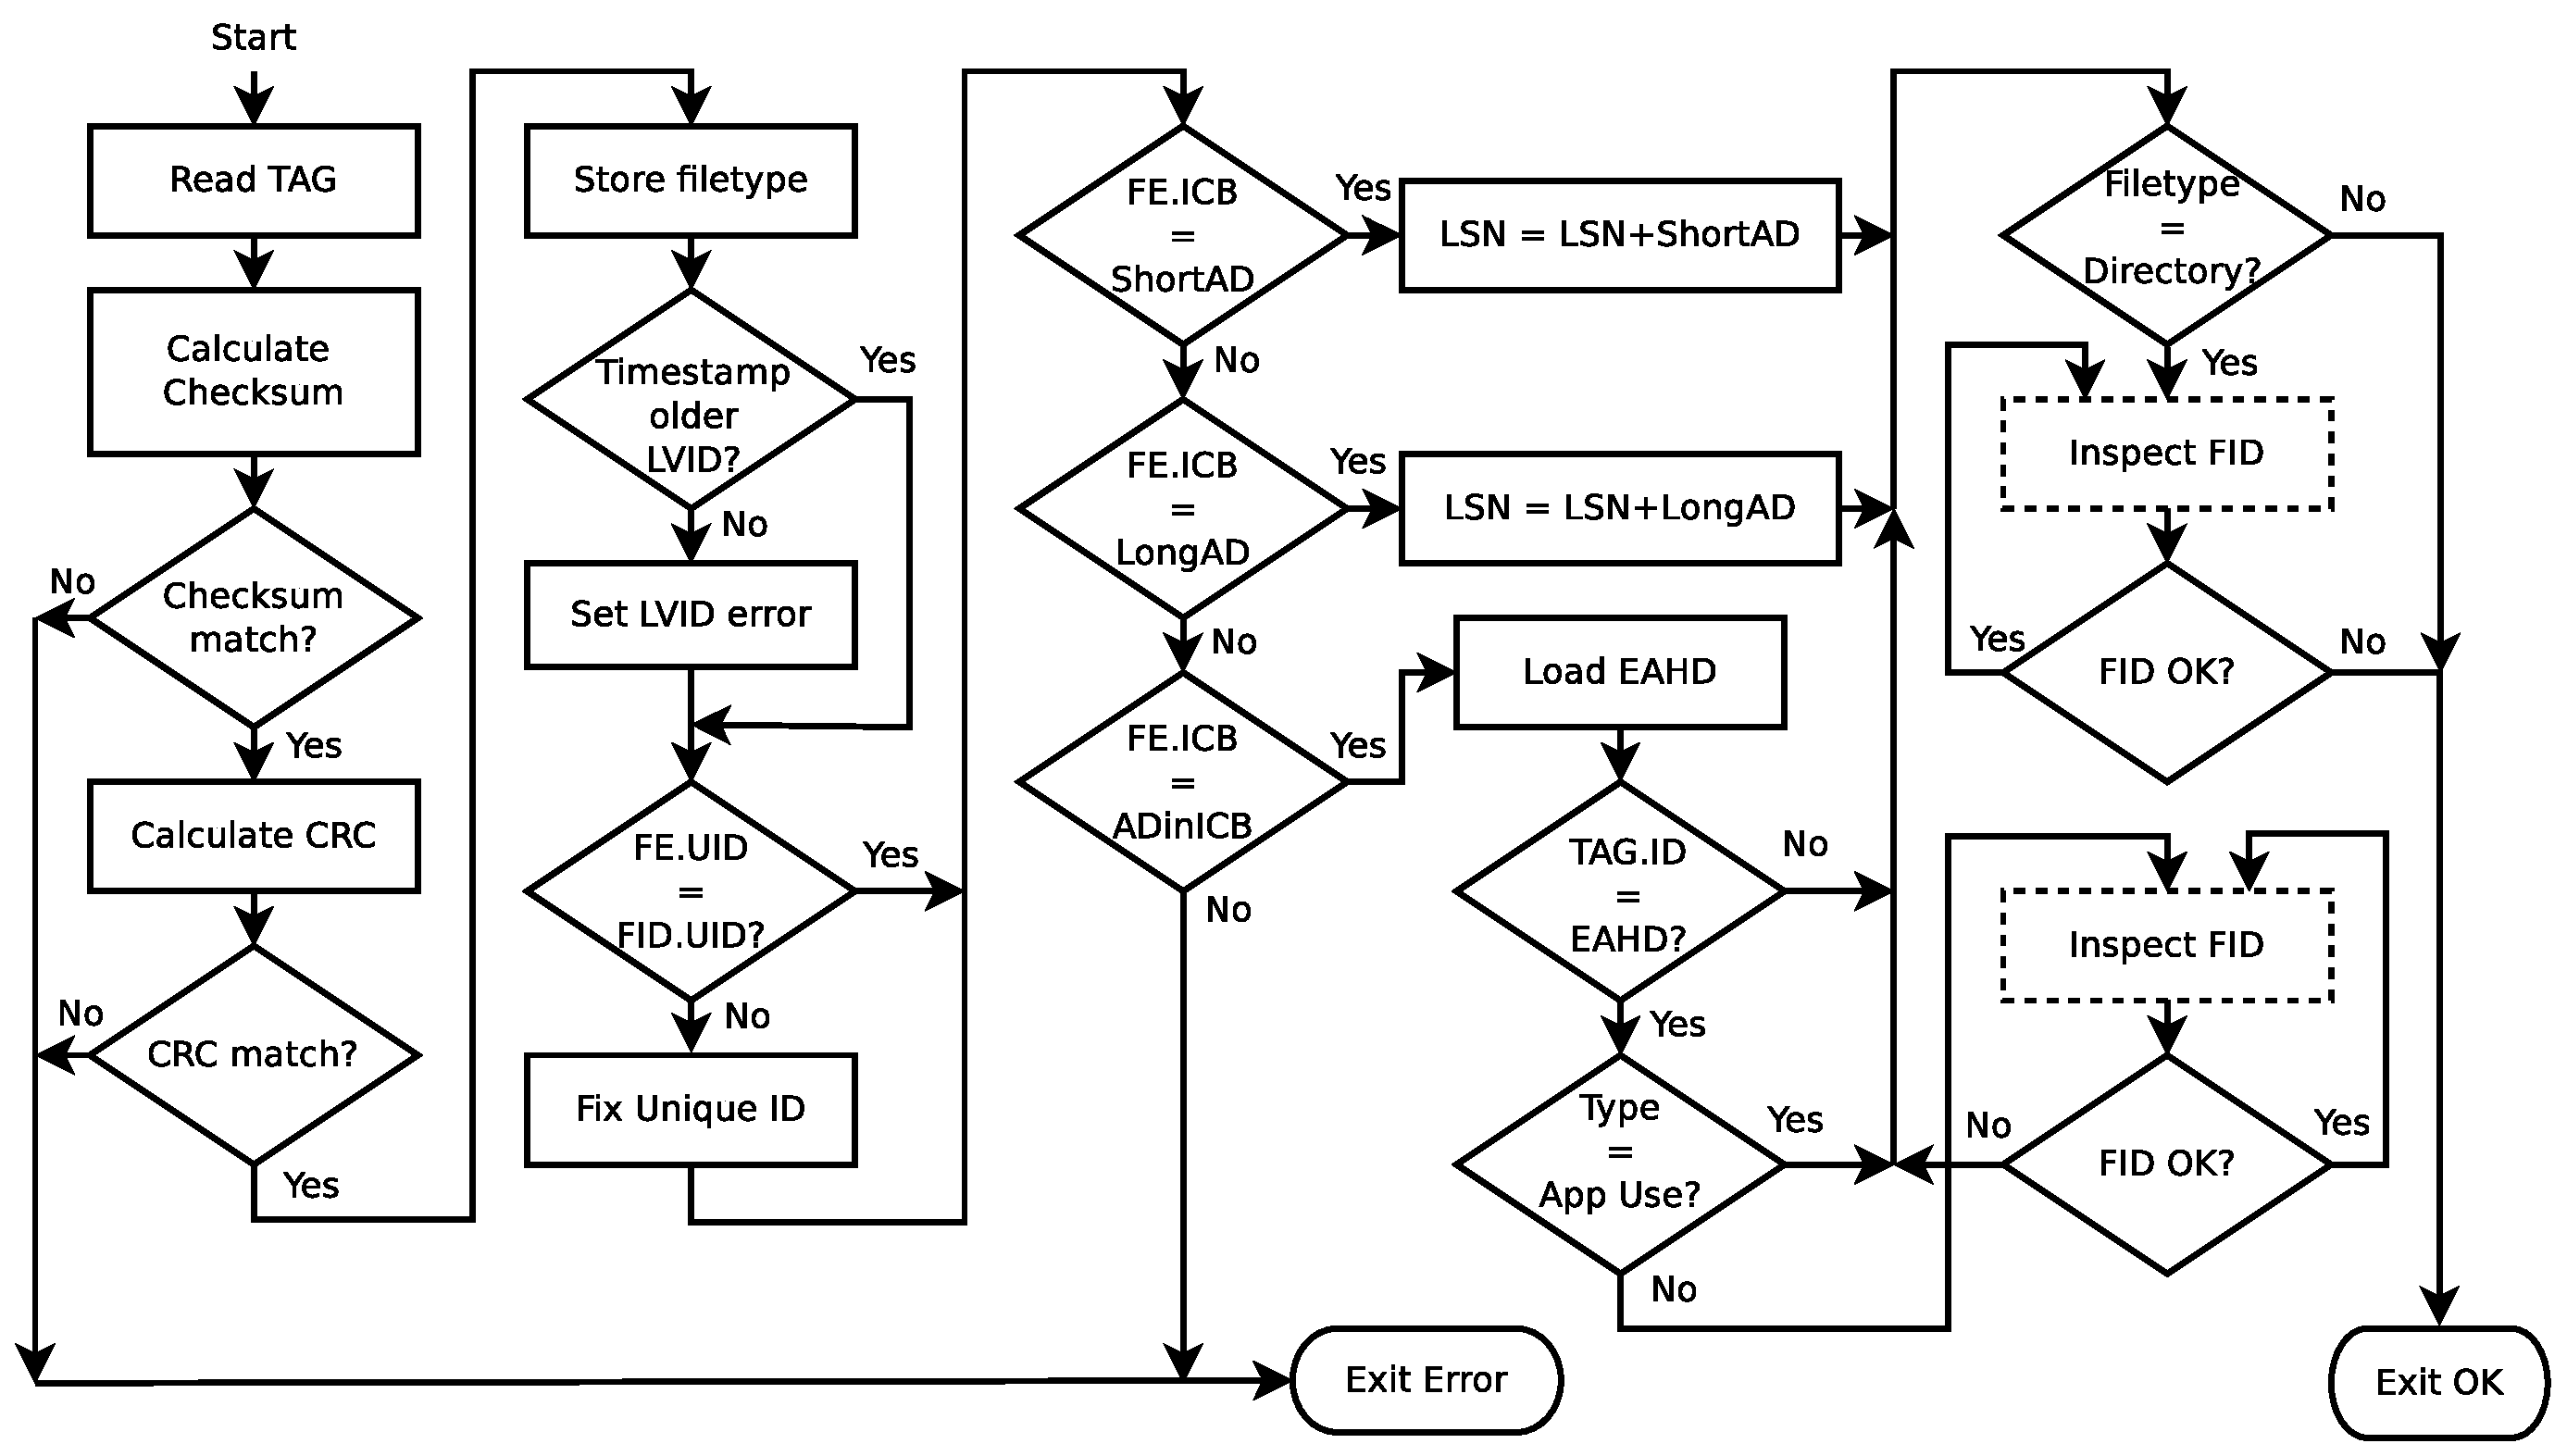
\includegraphics[scale=0.36]{obrazky/get-file.eps}
    \caption{Algoritmus načítání descriptorů FE (funkce \textit{Get File}). Tečkovaně naznačený blok odkazuje na obrázek \ref{fig:fid}.}
    \label{fig:files}
    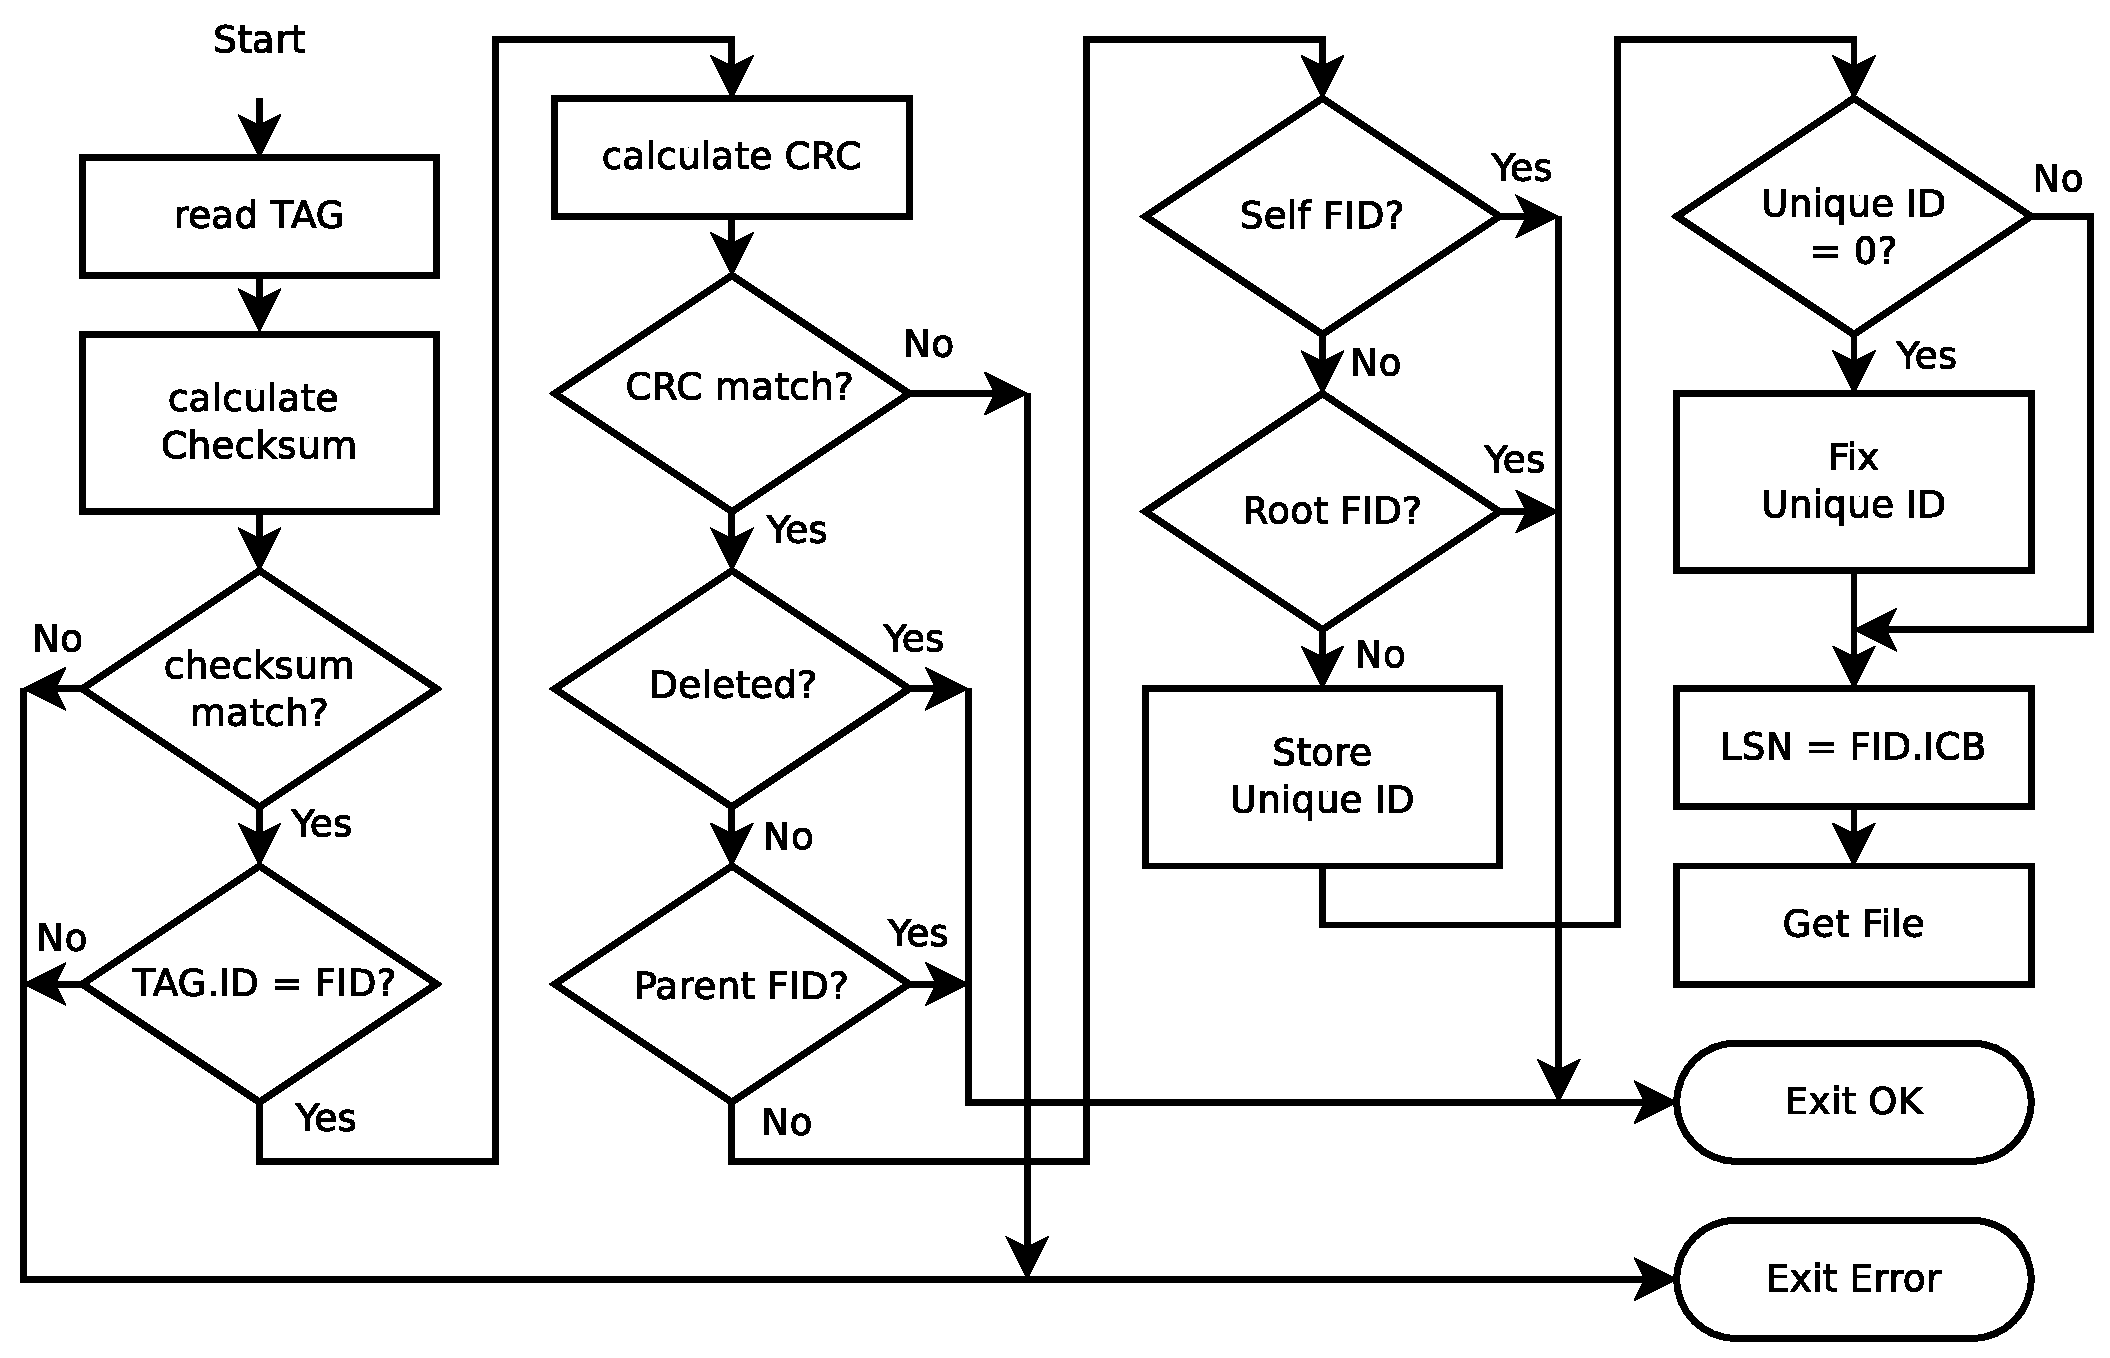
\includegraphics[scale=0.36]{obrazky/inspect-fid.eps}
    \caption{Algoritmus načítání descriptorů FID (funkce \textit{Inpspect FID}). Tečkovaně naznačený blok odkazuje na obrázek \ref{fig:files}.}
    \label{fig:fid}
\end{figure}

Algoritmus načtení adresářové struktury je zachycen na obrázku \ref{fig:files}. Tento algoritmus začíná po úspěšném načtení FSD, odkud je získána pozice FE kořenového adresáře, která je předána algoritmu. Od tohoto bodu probíhá algoritmus zachycený na obrázku. Předpokladem úspěšného průchodu je správnost všech kontrolních mechanismů. Ty není možné opravit, pouze je možné detekovat chybu. Ovšem pokud je deskriptor identifikován a selhala kontrola CRC, je uživateli v interaktivním režimu poskytnuta možnost tuto chybu ignorovat. Opravitelné chyby jsou chyby týkající se \textit{Unique ID} a časových značek. Po fázi detekce chyb následuje fáze hledání následující části stromu. Existuje několik druhů alokačních deskriptorů. Liší se způsobem jakým udržují informaci a kam mohou ukazovat. Povolené varianty jsou \textit{Long Allocation Descriptor} (LongAD), který ukazuje na logický blok v libovolném oddílu. \textit{Short Allocation Descriptor} (ShortAD) naopak může ukazovat na logický blok pouze ve svém oddílu. Poslední variantou je uložení deskriptorů FID přímo v FE (varianta ADinICB). Tato větev využívá volného místa, které vzniká za většinou deskriptorů, takže jsou FID uloženy přímo. Je zde použit deskriptor \textit{Extended Attribute Header Descriptor}, který v sobě nese buď nějaká implemenetační data, nebo sekvenci deskriptorů FID. Deskriptory FID jsou v obou případech procházeny iterativně dokud neskončí jeho načtení chybou (ať už protože je poškozený, tudíž není možné strom dále projít, nebo proto že sekvence skončila.) Zpracování samotných deskriptorů FID je popsáno ve vlastním algoritmu, který je na obrázku \ref{fig:fid}.

Algoritmus pro načítání deskriptorů FID je přímější. Začátek algoritmu je stejný jako v předchozím případě. Poté následuje sekvence dotazů, kdy nemá význam FID sledovat. Jedná se o příznak smazání, referenci na rodičovský adresář, sebe sama a kořenový adresář. Vzhledem k faktu, že chceme postupovat do hloubky, tyto reference nás nezajímají a proto algoritmus v tomto bodě končí (t.j. v algoritmu na obrázku \ref{fig:files} se přejde ke kontrole dalšího FID). Pokud touto částí algoritmus projde, přistoupí se k uložení aktuálního \textit{Unique ID} pro porovnání s FE a jeho kontrola na nulovost. Ta je případně opravena. Poté už následuje načtení pozice nového deskriptoru FE a jeho zpracování. Tím se algoritmus vrací opět k předchozímu algoritmu na obrázku \ref{fig:files}.

Během průchodu se sleduje několik parametrů, které jsou nutné ať už pro kontrolu a opravu stromu nebo pro opravu metadat v LVID \ref{sec:nacteni-a-oprava-lvid} a SBD \ref{sec:nacteni-a-oprava-sbd}. Jedná se o tyto:
\begin{itemize}
    \item Je \textit{Unique ID} nenulové (nulové musí být pouze pro kořenový adresář)?
    \item Je \textit{Unique ID} shodné pro FE a FID?
    \item Je \textit{Unique ID} menší než hodnota uložená v LVID?
    \item Jaký je čas poslední změny? Je tento čas později než je čas uložený v LVID? 
\end{itemize}
Pokud je kterýkoli dotaz zodpověděn záporně, je nastaven příznak chyby.

Další parametr, který sice není zachycen pro zachování jednoduchosti vývojového diagramu, je \textit{Tag Serial Number}. Jedná se o parametr, který slouží k opravě v případě katastrofické poruchy souborového systému a bylo by nutné jej zrekonstruovat. Je uložen v každém tagu souborového systému a pokud je tato možnost povolena (nemusí být), mají všechny stejnou hodnotu, která musí být 2 nebo větší. Tento údaj slouží k přiřazení daného tagu (a potažmo deskriptoru) ke správnému deskriptoru AVDP. Tím je vytvořen seznam deskriptorů, který je již možné rekonstruovat. Celý mechanismus je popsán ve specifikaci UDF \cite{osta-udf-0201}, kapitola 2.1.6.

Několikrát zmiňovaný je parametr \textit{Unique ID}. Jedná se o příznak, který je unikátní pro každý soubor nebo adresář. Je stejný pro FE a FID. Důvodem je šance na obnovu v případně katastrofického poškození souborového stromu. Pokud by se muselo přistoupit ke hledání jednotlivých FE ve všech sektorech logického svazku a párovat je s FID v adresářích, toto by byla jediná šance na obnovu.

Základním předpokladem pro použití tohoto algoritmu je ztráta některého z adresářů (například kořenového adresáře). To způsobí nemožnost načíst strom souborů z důvodu chybějícího vstupního bodu do stromu souborů. Nutno podotknout, že tento algoritmus není zahrnut v implementaci, ale jeho myšlenková struktura je následující:
\begin{enumerate}
    \item Díky známé velikosti logického bloku a známému umístění deskriptorů v nich (vždy na jeho začátku) lze procházet logickým svazkem po blocích a na každém se pokusit načíst \textit{File Entry} (FE) nebo \textit{Extended File Entry} (EFE), verifikovat jeho platnost pomocí jeho polohy, CRC a kontrolního součtu.
    \item Takto nalezený seznam FE a EFE bude vytvářet samostatné podstromy souborů (pokud médium obsahovalo další adresáře) a zbylé soubory bez rodičovského adresáře. Tato část probíhá podobně jako procházení stromem souborů, zkráceně takto:
    \begin{enumerate}
        \item Každý nalezený FE nebo EFE je klasifikován jako soubor nebo adresář. Pokud se jedná o adresář, je prohledán pro přítomnost \textit{File Identifier Descriptor} (FID). Pokud jsou nalezeny, dojde k pokusu spárovat je podle \textit{Unique ID} s ostatními nalezenými FE a EFE. Každý takto spárovaný FE (EFE) je vyřazen ze seznamu nalezených FE (EFE) a je zařazen do podstromu. Pokud se jedná o soubor, neděje se nic a pokračuje s k dalšímu nalezenému FE (EFE).
        \item Takto se vytvoří struktura podstromů a zbytku nezařazených FE a EFE.
    \end{enumerate}
    \item Nyní máme části původního stromu a zbytek FE (EFE). Ať už kořeny jednotlivých podstromů (nejvyšší adresář) nebo osamocené FE (EFE). Ty už není možné dále zařadit, proto budou zařazeny do chybějícího adresáře, který bude znovu vytvořen na místě původního. Jsou zde ovšem jistá omezení. Obnova není schopná zpětně získat názvy jednotlivých FE (EFE), protože ty jsou uloženy ve FID rodičovského adresáře. Stejně tak pokud by bylo nenávratně ztraceno více adresářů, nebylo by možné rozlišit, které FE (EFE) patří do kterého. 
\end{enumerate}
Jak je vidět ve výše popsaném algoritmu, obnova není absolutní, ale může poskytnout dobrý výchozí bod pro záchranu dat.

Důležitou částí, kterou je nutno popsat, je způsob vyřešení nedokončeného zápisu a způsoby jeho detekce. Vzhledem k faktu, že deskriptor LVID \ref{subsec:lvid} pomocí položky \textit{Integrity Type} pouze poukzauje, že médium nebylo korektně odebráno a ovladač může zaznamenat potřebné údaje o souboru dříve, než začne ukládat data, je potřeba mít způsob detekce této situace.

V tomto případě spoléháme na nekonzistentní deklarovaný objem uložených dat (položka deskriptoru FE \textit{Information Length}) a informaci o objemu skutečně uložených dat (položka deskriptoru FE \textit{Logical Blocks Recorded}), která by měla být aktualizována průběžně během, případně na konci zápisu. Ve chvíli, kdy se tyto údaje liší, soubor není kompletní.

V mé implementaci jsem zaujal přístup smazání daného souboru vzhledem k faktu, že informace kterou nese není kompletní. To je zajištěno označením daného souborou příznakem \textit{Deleted} v položce \textit{File Characteristics} v deskriptoru FID. Druhý úkol který je třeba v deskriptoru FID udělat je dle standardu ECMA-167\cite{ecma-167}, revize 3, kapitola 4/14.4.5, vynulování položky ICB, čímž se zajistí zničení reference pokud by při čtení nebyl kontrolován příznak smazání. Pro kompletnost byl vynulován celý deskriptor FE defektního souboru aby při případné obnově z katastrofického poškození nebyl mylně vyhodnocen jako platný. Takto vyřešený nedokončený zápis je viditelný při analýze souborového systému jako smazaný soubor a zároveň uživatel nenabývá mylného dojmu existence souboru, což byl efekt, který je patrný při použití nástroje v prostředí Microsoft Windows (nástroj \texttt{CHKDSK}).

\chapter{Výsledky a testování nástroje pro detekci a korekci chyb}
\label{ch:results}
%\todo{sepsat. popsat tesovaná data, jejich výrobu, objem (10 GB), výsledky, shrnout do grafu}
V této kapitole jsou popsána testovací data, metodika testování a dosažené výsledky. Kapitola je koncipována informativně a pracuje s vyběrovou množinou médií, která neobsahuje všechny možné varianty vzhledem k vysoké variabilitě UDF. Byl zvolen přístup otestování vůči nejběžnějším variantám médií, což bývá výchozí nastavení nástrojů pro vytvoření UDF, obvykle se lišící pouze nosným médiem, velikostí bloku a verzí UDF. Toto bylo ověřeno vůči médiím, které vznikly na platformách \mbox{GNU/Linux}, Microsoft Windows a Apple macOS. 

\section{Testovací data}
\label{sec:data}
Testovacími daty jsou myšlena různá média, která jsou naformátována souborovým systémem UDF. Tato média různých parametrů jsou záměrně poškozována a následně analyzována.

Testovací sada obsahuje média všech povolených velikostí sektorů (t.j od 512~B do 4096~B) a různých verzí (od 1.02 do 2.60 přičemž většina testů je mířena proti 2.01.) Poškozování médií probíhalo dvěma způsoby: synteticky a nahodile.

Syntetické poškození média probíhalo ručním přepsáním některých vybraných částí média pro vytvoření chyby v daném deskriptoru. Takto byly testovány kontrolní součty a CRC a posléze opravy takto poškozených deskriptorů.
Nahodilé poškození média bylo vytvořeno záměrným přerušením zápisu na médium odebráním zařízení. Nahodilé proto, že není předem jasné, co bude poškozeno a jak. Tyto testy cílí na obnovu stromu souborů a opravu a uzavření LVID.

Tímto způsobem bylo vytvořeno přes 14~GB testovacích dat ve 29 vzorcích.

Pro zjištění chyb na médiích a pro zjištění úspěšnosti detekce a následné korekce byl použit nástroj společnosti Philips \texttt{udfct} \cite{wayback} určený ke kontrole dodržování standardu UDF.

\section{Metodika testování}
\label{sec:metodika}
Metodika testování je navržena následovně:
\begin{enumerate}
    \item Vytvoří se čerstvá kopie testovacích dat.
    \item Spustí se referenční nástroj \texttt{udfct} \cite{wayback} pro zjištění aktuálního stavu média pro následné srovnání.
    \item Spustí se nástroj \texttt{udffsck} v kontrolním režimu a porovnají se výstupy s referencí.
    \item Pokud médium obsahuje chyby, spustí se nástroj \texttt{udffsck} v opravném režimu.
    \item Nástroj \texttt{udffsck} je spuštěn opět v kontrolním režimu. Pokud došlo v předchozím kroku k plné opravě (návratová hodnota 1), mělo by médium být nyní bez chyb (návratová hodnota 0)
    \item Spustí se referenční nástroj \texttt{udfct} a opět se porovnají výstupy. Pokud byla oprava úspěšná, médium by nemělo nyní vykazovat chyby, nebo pokud chyby vykazuje, neměly by ovlivňovat funkci souborového systému.
\end{enumerate}
Tato metodika byla navržena pro potřeby vývoje nástroje a pro zajištění maximálního možného pokrytí případných chyb média (obzvláště u nahodile poškozených médií.) Zjednodušená verze tohoto testu byla implementována pro potřeby automatického testování službou Travis CI. Ta je omezena pouze na testování vlastního nástroje bez reference a testuje vůči předpokládaným návratovým hodnotám. V principu jde o vynechání kroků 2 a 6 z předchozí sekvence.

Tento přístup pomohl odhalit řadu potíží během vývoje, kdy opravením jedné chyby byla vytvořena omylem chyba jiná. Takto byla chyba podchycena okamžitě po vzniku, takže mohla být okamžitě vyřešena bez opakované analýzy problému. 

\section{Srovnání s ostatními řešeními}
\label{sec:srovnani}
\begin{figure}[] 
    \centering
    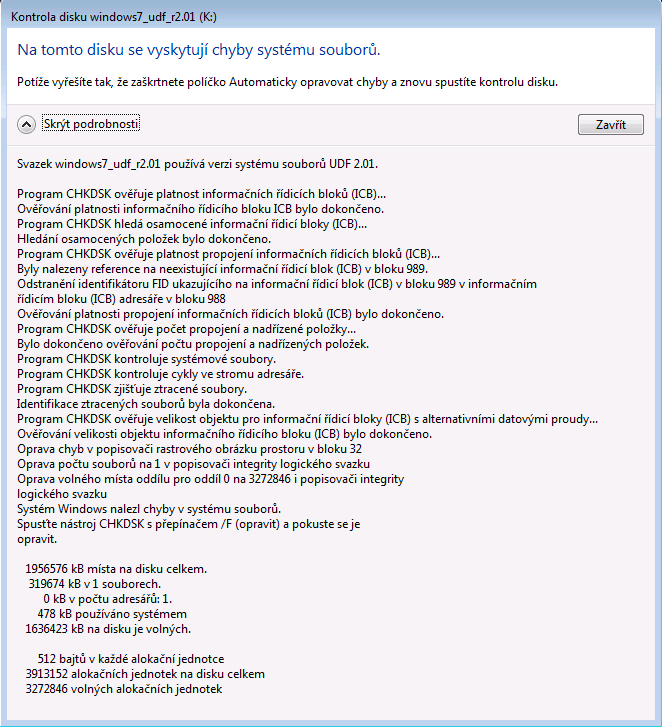
\includegraphics[scale=0.38]{obrazky/chkdsk.png}
    \caption{Výsledek kontroly poškozeného média nástrojem \texttt{CHKDSK}}
    \label{fig:chkdsk}
\end{figure}
Pro ověření správné funkce nástroje byla vybraná média otestována i na jiných operačních systémech pro srovnání funkce. Jako ukázku tohoto přístupu lze zvolit médium, které vzniklo na MS~Windows pro flash disk (tedy \textit{Overwritable} médium) a následně bylo záměrně poškozeno přerušením zápisu.

Byla provedena kontrola disku na MS~Windows~7 pomocí nástroje \textit{CHKDSK}. Výsledek jeho kontroly před jakoukoli opravou je na obrázku \ref{fig:chkdsk}. Kontrola byla provedena i na MS~Windows~10 se stejným výsledkem. Podle nástroje \texttt{CHKDSK} je médium opravitelně poškozeno.

Podobný výsledek byl získán v Apple macOS programem \texttt{fsck\_udf}. Přepis jeho výstupu je ve výpisu v příloze \ref{lst:fsck-udf-mac}. Z obou výstupů je vidět, že oba nástroje došly ke stejným poruchám na médiu.
Médium bylo v této fázi zazálohováno pro srovnání různých variant. První varianta je oprava pomocí mého nástroje \texttt{udffsck}. Druhá varianta je oprava pomocí nástroje MS~\texttt{CHKDSK}. Oprava pomocí \texttt{fsck\_udf} z Apple macOS není možná, protože nástroj nemá implementovány žádné opravné algoritmy. Pro referenční srovnání je přiložen výstup z programu \texttt{udfct} společnosti Philips, jehož výstup je vzhledem k jeho délce v příloze \ref{lst:udfct-broken}.

\begin{lstlisting}[frame=single,caption={Výsledek opravy poškozeného média programem \texttt{udffsck}},label=lst:udffsck-pass,basicstyle=\ttfamily\scriptsize, keywordstyle=\color{black}\bfseries\underbar,nolol,numbers=left,texcl=false,escapechar=!]
Verbosity increased to WARNING.
Verbosity increased to MESSAGE.
We try to fix medium automaticaly.
Medium to analyze: /dev/sdb
AVDP[0] successfully loaded.
AVDP[1] successfully loaded.
AVDP[2] successfully loaded.
Sectorsize: 512

Medium file tree
----------------
.....:..rwx.:.rwx.:.rwx DIR     2017-05-05 15:58:54.804378+00:00       152  <ROOT>
  .....:..rwx.:.rwx.:.rwx FILE    2009-11-12 19:46:14.000000+00:00  327345425  "gtd.mp4"
!\colorbox{yellow}{[ERROR] (2017-01-16-191632.webm) Tag Serial Number differs.}!
!\colorbox{green}{(2017-01-16-191632.webm) Tag Serial Number was fixed.}!
!\colorbox{yellow}{[ERROR] (2017-01-16-191632.webm) File size mismatch. Probably unfinished file write.}!
!\colorbox{green}{Removing unfinished file...}!
!\colorbox{green}{(2017-01-16-191632.webm) Unifinished file was removed.}!

Filesystem status
-----------------
Volume set identifier:113A1E01 UDF Volume Set
Partition identifier:
Next UniqueID: 18
Max found UniqueID: 17
Last LVID recoreded change: 2017-05-05 16:15:01.278032+00:00
expected number of files: 2
expected number of dirs:  1
counted number of files: 1
counted number of dirs:  1
UDF rev: min read:  0201
         min write: 0201
         max write: 0201
Used Space: 327836672 (640306)
Free Space: 1665865216 (3253643)
Partition size: 2003533824 (3913152)
Expected Used Space: 337668608 (659509)
Expected Used Blocks: 882490
Expected Unused Blocks: 3030662
!\colorbox{yellow}{[ERROR] 19203 blocks is unused but not marked as unallocated in Free Space Table.}!
!\colorbox{yellow}{[ERROR] Correct free space: 3272846}!
!\colorbox{yellow}{[ERROR] 242184 blocks is unused but not marked as unallocated in SBD.}!

VDS verification status
-----------------------
[0] PVD is fine. No fixing needed.
[1] PD is fine. No fixing needed.
[2] LVD is fine. No fixing needed.
[3] USD is fine. No fixing needed.
[4] IUVD is fine. No fixing needed.
[5] TD is fine. No fixing needed.
!\colorbox{yellow}{[ERROR] Opened integrity type. Some writes may be unfinished.}!
!\colorbox{yellow}{[ERROR] Number of files or directories is not corresponding to counted number}!
!\colorbox{yellow}{[ERROR] Free Space table is not corresponding to reality.}!
!\colorbox{green}{PD SBD recovery was successful.}!
!\colorbox{green}{LVID recovery was successful.}!
All done
\end{lstlisting}
\begin{figure}[b] 
    \centering
    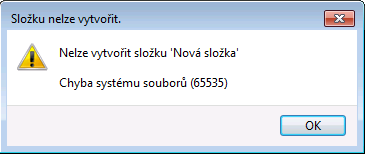
\includegraphics[scale=0.42]{obrazky/win7-error.png}
    \caption{Chyba při pokusu o zápis na médium opravené nástrojem \texttt{CHKDSK}}
    \label{fig:win7-err}
\end{figure}
Výsledek z nástroje \texttt{udffsck} je vidět na výpisu \ref{lst:udffsck-pass}. Jak je vidět, byla nalezena řada chyb a všechny byly opraveny. Funkčnost souborového systému byla posléze ověřena připojením k MS~Windows~7, kde na něj byla úspěšně nakopírována data. Stejně tak výstup z programu MS~\texttt{CHKDSK} nedetekoval žádné problémy. Nabízí se otázka, proč nebyla funkce souborového systému ověřena i na OS~Linux. Důvodem je benevolence implementace ovladače v OS~Linux, který dokáže bez potíží zapisovat i na defektní souborový systém. Problém je, že ho tím dále poškozuje. Proto byl jako kontrolní test zvolen MS~Windows~7, který přistupuje k připojení souborového systému striktněji.

Nyní pokud se vrátíme k zálohované variantě a zkusíme pro srovnání provést obnovu pomocí MS~\texttt{CHKDSK}. Na konci opravy, kdy program hlásí, že opravil všechny nalezené chyby, zkusíme taktéž médium připojit a nahrát data. Nyní ale dochází k selhání, viz obrázek \ref{fig:win7-err}. Opětovná kontrola pomocí \texttt{CHKDSK} nenalezne žádné chyby. Verdikt je, že médium je nenávratně poškozeno, ačkoli \texttt{CHKDSK} nenalézá chybu. Po kontrole referenčním nástrojem \texttt{udfct}, jehož výstup je opět v příloze \ref{lst:udfct-chkdsk}, je vidět, že program \texttt{CHKDSK} sice opravil nalezené chyby, ale také vytvořil nové. K jeho opravě by bylo nutné částečné přeskupení struktur na médiu, což ostatně svým během udělal a právě tím médium poškodil, protože tak neprovedl v souladu se specifikací. Pokud použijeme můj nástroj \texttt{udffsck}, zjistíme, že někeré z chyb jsou opravitelné, ale jejich odstranění vyvolává další, které můj nástroj již bohužel nedetekuje. Jejich nález je opět díky \texttt{udfct}, jehož výpis je v příloze \ref{lst:udfct-chkdsk-po-oprave}. Ovšem na rozdíl od chyb, které vytvořil program \texttt{CHKDSK}, nemají mnou vytvořené chyby dopad na funkci souborového systému, to dokazuje i opětovný pokus o připojení a nahrávání dat na MS~Windows~7, který nyní neselže.

Cílem této analýzy bylo ukázat, že nástroj \texttt{udffsck} dokáže opravit poškozený souborový systém UDF tak, že i striktní ovladač MS~Windows dokáže bez potíží s médiem pracovat na rozdíl od jejich vlastního řešení \texttt{CHKDSK}. Vzhledem k faktu, že neexistuje jiné řešení, ať už otevřené nebo uzavřené, schopné jak detekce chyb, tak jejich korekce pro souborový systém UDF, považuji tento výsledek za úspěch. 

\section{Dosažené výsledky}
\label{sec:vysledky}
Byl vytvořen a otestován nástroj, který implementuje jak detekční, tak korekční algoritmy pro souborový systém UDF. Jeho funkce byla ověřena jak praktickým používáním na poškozená média, tak porovnáním výsledků detekce a následné korekce vůči ostatním existujícím řešením.

K vytvoření nástroje byl použit programovací jazyk C ve standardu C99 s použitím knihovních funkcí GNU/Linux. Jsou využívány výhradně funkce poskytované API GNU/Linux, což snižuje nároky na přeložení pro danou distribuci. Výčet požadovaných funkcí a knihoven je tento: \texttt{install}, \texttt{gawk}, \texttt{make}, \texttt{gcc} (nebo \texttt{clang}), \texttt{sed}, \texttt{grep}, \texttt{ld}, \texttt{nm}, \texttt{objdump}, \texttt{ar}, \texttt{ar}, \texttt{strip}, \texttt{ranlib}, \texttt{mt}, \texttt{ncurses}, \texttt{libreadline}, \texttt{libtool}, \texttt{automake}, \texttt{autoheader}, \texttt{autoconf}.

Nástroj v tuto chvíli implementuje podporu standardů UDF 1.00 až 2.01, přičemž většina vývoje byla soustředěna na novější verzi standardu. Proti tomu stojí nedostatek testovacích médií vůči kterým bylo zařízení testováno. Uměle vytvořená média (myšleno vytvořená pro účely testování) mají sice známou minulost ale to je částečně na škodu vzhledem k faktu, že opravdu závažné chyby vzniknou až během provozu média delší dobu.

Nástroj v tuto chvíli dokáže detekovat a opravovat chyby podle tabulky \ref{tab:det-cor}. Chyba, ochranný mechanismus nebo funkce UDF, která není zachycena v této tabulce, není detekována.
\begin{table}[h]
    \centering
    \begin{tabular}{ | l | l | l | }
        \hline
        Název chyby & Detekce & Korekce \\ \hline\hline
        Neshodující se kontrolní součet & \cmark & \cmark (\footnotemark[1]) \\\hline
        Neshodující se CRC & \cmark & \cmark (\footnotemark[1]) \\\hline
        Neshodující se umístění tagu & \cmark & \cmark \\\hline
        Neshodující se počet souborů nebo adresářů & \cmark (\footnotemark[2]) & \cmark (\footnotemark[2]) \\\hline
        Neshodující se objem volného místa & \cmark (\footnotemark[2]) & \cmark (\footnotemark[2]) \\\hline
        Neshodující se mapy obsazeného místa & \cmark (\footnotemark[2]) & \cmark (\footnotemark[2]) \\\hline
        Špatně nastavené \textit{Unique ID} & \cmark & \cmark \\\hline
        Špatně nastavené časové značky modifikace & \cmark & \cmark \\\hline
        Špatně nastavené časové značky vytvoření & \xmark (\footnotemark[4]) & \xmark (\footnotemark[4]) \\\hline
        Rozdílné \textit{Tag Serial Number} & \cmark & \cmark \\\hline
        Uzavření otevřeného deskriptoru LVID & \cmark & \cmark \\\hline
        Vyřešení nedokončeného zápisu & \cmark & \cmark \\\hline
        Poškozený deskriptor FE & \cmark & \xmark (\footnotemark[3]) \\\hline
        Poškozený deskriptor FID & \cmark & \xmark (\footnotemark[3]) \\\hline
        Poškozený deskriptor FSD & \cmark & \xmark (\footnotemark[3]) \\\hline
    \end{tabular}
    \caption{Tabulka detekovatelných a opravitelných chyb\label{tab:det-cor}}
\end{table}

\footnotetext[1]{Pokud došlo k této poruše u redundantního deskriptoru}
\footnotetext[2]{Závislé na správnosti průchodu stromem souborů}
\footnotetext[3]{Oprava je sice technicky možná přepisem na správné hodnoty, ale není možné automaticky usoudit zda je při použití vadného deskriptoru v pořádku pokračovat. Tato možnost musí být svěřena pouze uživateli.}
\footnotetext[4]{Nebylo implementováno. Jedná se o porovnání pořadí času vytvoření a poslední modifikace.}

\chapter{Publikace nástroje v GNU komunitě}
\label{ch:publikace}
Publikace v GNU komunitě proběhla díky začlenění vývojové větve zpět do zdrojového balíčku \texttt{udftools}. Předpoklady a kroky vedoucí k úspěšnému začlenění včetně dopadu po začlenění jsou popsány v následujících sekcích.

\section{Integrace do balíčku \texttt{udftools}}
\label{sec:integrace}
Proces integrace do zdrojového balíčku je důležitou částí práce. Bez ní zůstane má práce pouze jako vývojová větev a nikdy se nedostane k uživatelům. Proto byla na začátku práce navázána komunikace s aktuálním správcem balíčku \texttt{udftools}, panem Palim Rohárem, který vlastní repozitář balíčku.

Vzhledem k nízké aktivitě ze strany vývojářů na balíčku \texttt{udftools} neexistuje seznam požadavků pro přispívání do balíčku, jako to je u jiných (aktivnějších) projektů. Tyto požadavky byly vyjednány s panem Rohárem a jednalo se o tyto:
\begin{itemize}
    \item Funkční řešení přeložitelné pomocí GCC s využitím GNU Autotools. 
    \item Kód okomentovaný a náležitě zdokumentovaný pro budoucí udržování.
    \item Vytvoření testů pro otestování funkčnosti v budoucnosti. Není potřeba vytvářet unit testy, ačkoli jsou vítány.
    \item Vytvoření manuálové stránky k programu.
\end{itemize}
Protože vývoj probíhá na serveru GitHub, samotná práce probíhala ve vlastní větvi, která vznikla rozdělením od původního projektu (\textit{Fork}) a opačný proces, který větev začlení zpět, je nazýván \textit{Pull Request}. To znamená, že vlastník repozitáře je vyzván ke sloučení vývojové větve s hlavní (\textit{Merge}). To může proběhnout bez konfliktů, což je ideální stav, nebo dojde ke konfliktu se změnami v hlavní větvi. Pokud jsou konflikty vyřešeny a změny odpovídají požadavkům vlastníka repozitáře, změny jsou začleněny a vývojová větev je integrována. 

\section{Dopad integrace do balíčku \texttt{udftools}}
\label{sec:dopad}
Práce na \texttt{udffsck} byla od počátku koncipována jako součást existujícího balíčku \texttt{udftools}. Ten je začleněn ve většině distribucích GNU/Linux, potíž je, že často ve starých verzích, které jsou navázané na starý repozitář \cite{udftools-sourceforge} místo stávajícího \cite{udftools-github}.

Pokud bychom tedy přepokládali integraci pouze do distribucí, které aktuálně používají verzi z nového repozitáře \texttt{udftools}, získali bychom tento seznam:
\begin{itemize}
    \item\textbf{Debian} -- aktuálně je balíček ve verzích Debian Testing a Debian Unstable. Více v \cite{udftools-debian}.
    \item\textbf{Gentoo} -- starší verze balíčku je v tuto chvíli Stable, poslední vydaná je Testing. Více v \cite{udftools-gentoo}.
    \item\textbf{Arch Linux} -- balíček je dodáván pomocí komunitního repozitáře AUR \cite{udftools-arch}.
    \item\textbf{Ubuntu} -- balíček je dodáván pomocí PPA. Je podporován ve verzích Ubuntu Zesty a Ubuntu Artful \cite{udftools-ppa}.
    \item\textbf{Fedora, Red Hat Enterprise} -- poslední verze Fedora Linux obsahuje i poslední vydanou verzi balíčku, takže lze předpokládat její napojení na repozitář. Pravděpodobně bude tento balíček předáván i do RHEL, protože je známa aktivita v repozitáři ze strany společnosti Red Hat.
    \item\textbf{OpenSuse} -- tato distribuce má v oficiálních repozitářích starou verzi balíčku, ale v \cite{udftools-rpm} je k dispozici předkompilovaný balíček.
\end{itemize}
Jak je vidět, po začlenění se nástroj \texttt{udffsck} poměrně rychle dostane ke svým uživatelům skrz oficiální nebo komunitní distribuční kanály.

Dalšími kroky po úspěšné integraci bude průzkum pro další rozvoj nástroje. Prvními kroky pravděpodobně bude rozšíření podpory pro novější verze UDF. To bude pravděpodobně vyžadovat širší záběr než jen práci na \texttt{udffsck}, protože bude nutné přidat nové funkce z novějších verzí standardu UDF do sdílených hlavičkových souborů, což ovlivní i zbytek nástrojů v balíčku.
